\documentclass[final,twocolumn,5p]{elsarticle}
\usepackage{times}
\usepackage{blindtext, graphicx}
\usepackage{subfigure}
\usepackage{colortbl}
\usepackage{cleveref}
\usepackage{tikz}
\def\firstcircle{(90:1.75cm) circle (2.5cm)}
\def\secondcircle{(210:1.75cm) circle (2.5cm)}
\def\thirdcircle{(330:1.75cm) circle (2.5cm)}

\usepackage{balance}
\definecolor{Gray}{rgb}{0.88,1,1}
\definecolor{Gray}{gray}{0.85}
\definecolor{lightgray}{gray}{0.8}
\usepackage[framed]{ntheorem}
\usepackage{framed}
\usepackage{tikz}
\usetikzlibrary{shadows}
\theoremclass{Lesson}
\theoremstyle{break}

% inner sep=10pt,
\tikzstyle{thmbox} = [rectangle, rounded corners, draw=black,
fill=Gray!20,  drop shadow={fill=black, opacity=1}]
\newcommand\thmbox[1]{%
    \noindent\begin{tikzpicture}%
    \node [thmbox] (box){%
        \begin{minipage}{.94\textwidth}%
        \vspace{-3mm}#1\vspace{-3mm}%
        \end{minipage}%
    };%
    \end{tikzpicture}}

\let\theoremframecommand\thmbox
\newshadedtheorem{lesson}{Finding}
\newcommand{\quart}[4]{\begin{picture}(80,4)%1
    {\color{black}\put(#3,2){\circle*{4}}\put(#1,2){\line(1,0){#2}}}\end{picture}}

%% space saving measures
% \usepackage[shortlabels]{enumitem}  
% \usepackage{url}

\begin{document}

% \pagenumbering{arabic} %XXX delete before submission

\begin{frontmatter}
  \title{ How to Read Less:\\ Better Machine Assisted Reading Methods for Systematic Literature Reviews}
\author[add1]{Zhe Yu\corref{cor1}}
\ead{zyu9@ncsu.edu}
\author[add2]{Nicholas A. Kraft}
\ead{nicholas.a.kraft@us.abb.com}
\author[add1]{Tim Menzies}
\ead{tim.menzies@gmail.com}
\cortext[cor1]{Corresponding author.}
\address[add1]{Department of Computer Science, North Carolina State University, Raleigh, NC, USA}
\address[add2]{ABB Corporate Research, Raleigh, NC, USA}


\begin{abstract}
  
\noindent\textbf{Context:} Systematic literature reviews (SLRs) are the primary method for aggregating and synthesizing evidence in evidence-based software engineering. Primary study selection is a critical and time-consuming SLR step in which reviewers use
titles, abstracts, or even full texts to evaluate thousands of studies to find
the dozens of them that are relevant to the research questions. \\
\textbf{Objective:} We seek to reduce the effort of primary study selection in SLRs with machine assisted reading techniques.\\
\textbf{Method:} In this paper we explore and refactor the state-of-the-art machine assisted reading techniques from both evidence-based medicine and legal electronic discovery to support SLRs. By refactoring those methods, we discovered FASTREAD, which is a new state-of-the-art in machine assisted reading for SLRs. Tested on two data sets generated from existing SLRs of Hall, Wahono, et al., FASTREAD outperforms the current state-of-the-art methods.\\
\textbf{Results:} Using FASTREAD, it is possible to find $90\%$ of the studies found by standard manual methods, but after only reading less than $10\%$ of the candidate studies. \\
\textbf{Conclusions:} With the help of FASTREAD, conducting an SLR is much more
efficient and less difficult. Software Engineering researchers now have no excuse: they should conduct SLRs.

\end{abstract}
\end{frontmatter}


 
\vspace{1mm}
\noindent
{\bf Keywords:} Active Learning, Machine Assisted Reading, Systematic Literature Review, Software Engineering.
%  \maketitle 

\section{Introduction}
\label{sect: Introduction}

 The
number of new publications every year is growing rapidly. For example, on defect
prediction, 729 studies were published on IEEE
Xplore\footnote{http://ieeexplore.ieee.org} during the year of 2005 while 1,564
studies were published during the year of 2015.
Given this increasingly faster pace of software engineering (SE) research,
it has become harder and harder to remain current with
the state-of-the-art research in software engineering.

Systematic Literature Reviews
(SLRs) are one approach to this problem. SLRs are a well established and widely
applied review method in Software Engineering since Kitchenham, Dyb{\^{a}}, and
J{\o}rgensen first adopted it to support evidence-based software engineering in
2004 and 2005~\cite{kitchenham2004evidence,1377125}. 
Researchers can get a
general idea of current activity in their field of interests by reading the SLR
studies. Furthermore, a
deeper understanding of the topic may be gained by conducting an SLR.

An increasing number of SLRs has been conducted since the proposal and
revision of the SLR guidelines by Kitchenham in 2007~\cite{keele2007guidelines}. For
example, there are 26 SLRs on IEEE Xplore during the year of 2005 and the
number has increased to 137 for the year of 2010 and 199 for the year of
2015. Various scholars  suggest that an SLR is required before any research in Software
Engineering is conducted~\cite{keele2007guidelines}.
While this is certainly a good advice,
currently an SLR is
a large, time consuming and complex
task~\cite{hassler2016identification,hassler2014outcomes,carver2013identifying,bowes2012slurp}.

The
goal of our research is to reduce the effort of an SLR to days of work and
make it practical to be conducted frequently.
Previously we have analyzed the costs of SLRs~\cite{hassler2014outcomes,carver2013identifying}. As shown in Figure~\ref{fig:barrier}, primary study selection, which is noted as ``selecting papers'' in Figure~\ref{fig:barrier}, is among the top three most difficult
as well as time-consuming aspects in an SLR. Usually, reviewers need to evaluate
thousands of studies trying to find dozens of them that are relevant to the
research questions based on their title, abstract, or full text~\cite{bowes2012slurp}. An extreme
example of this is where reviewers sourced over
3,000 studies, and only used 7 of them in their final review~\cite{bezerra2009systematic}. The cost associated with primary study selection has become a
serious problem and will continue to grow in the near future
 as the population of candidates for primary
studies increases dramatically.


\begin{figure*}[ht]
    \centering
    \subfigure[Most Difficult Aspects of SLR Process.]
    {
        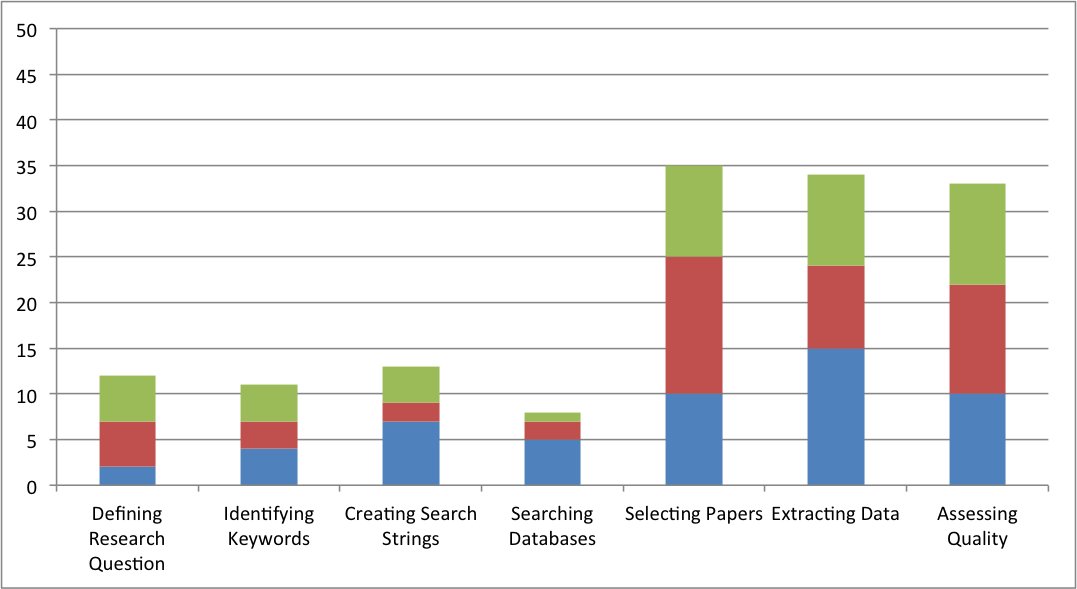
\includegraphics[width=0.48\linewidth]{difficult.png}
        \label{fig: difficult}
    }
    \subfigure[Most Time Consuming Aspects of SLR Process.]
    {
        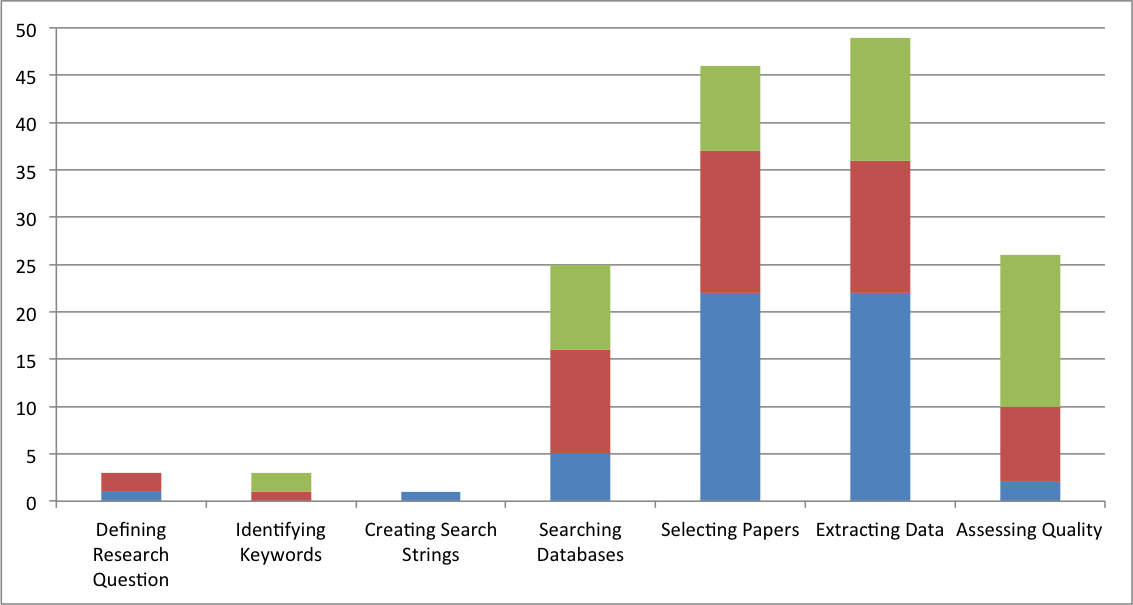
\includegraphics[width=0.48\linewidth]{time.png}
        \label{fig: time}
    }    
    \caption{Data collected from surveys to SLR authors~\cite{carver2013identifying}. Measured by number of votes, where blue, red, and green are number of times voted as most, second most, and third most, respectively.}
    \label{fig:barrier}
\end{figure*}


The problem of how to read more materials, faster, has been studied by many fields.
Researchers in evidence-based medicine rely on extensive reading studies in order
to survey their field~\cite{wallace2010semi,wallace2010active}.
Also, researchers exploring ``electronic discovery''
have developed algorithms  to quickly discover what documents
are most relevant to a particular legal
summons~\cite{cormack2014evaluation,cormack2015autonomy}.

The goal of this paper is to check if any of those methods
from other fields can assist SLRs in software engineering.

%
To accomplish this, we explored
state-of-the-art methods in machine assisted reading from  medical and legal domains.
It turns out, those methods were not exactly suited to SLRs for SE.
However, by breaking them apart and refactoring them, we created FASTREAD,
a new state-of-the-art method for machine assisted SLRs in software engineering.
We recommend FASTREAD because:
\begin{itemize}

  \item Using FASTREAD, 90\% of the ``relevant'' studies can
  be retrieved by reviewing only 10\% of the candidate studies. That is,
  FASTREAD can significantly reduce the cost of SE SLRs.
  \item On SE SLRs, FASTREAD performs remarkably better than state-of-the-art
  methods from medical and legal domains.
\end{itemize}
The rest of this paper defines and refactors machine assisted reading techniques
from evidence-based medicine~\cite{wallace2010semi,wallace2010active} and
electronic discovery~\cite{cormack2014evaluation,cormack2015autonomy}.
To assess our newly refactored methods,
we need some ``gold sets'',
against which we can compare different methods. Fortunately, in the arena of software
engineering, there exist very prominent ``gold sets'' as published SLRs. This paper explores two such SLRs: Wahono et al. 2015~\cite{wahono2015systematic} and Hall et
al. 2012~\cite{hall2012systematic}.  We choose these since they seem to be the
state-of-the-art in this arena. One is very recent (2015), the other is highly
cited (305 citations), and both define their work in enough details for us to try to
reproduce their results using automatic methods. More details about the ``gold
sets'' will be presented later in Section~\ref{sect: Data Sets}. Using
these ``gold sets'', we ask and answer the following four research questions:

\begin{itemize}

\item
{\bf RQ1: What are the costs of a standard SLR primary study selection?} According to our literature survey, it usually requires months of tedious work for a standard SLR primary study selection.

\item
{\bf RQ2: What are the state-of-the-art machine assisted reading methods?} The
state-of-the-art machine assisted reading techniques are patient active learning
from evidence-based medicine and continuous active learning from electronic
discovery. These two methods are explained later in Section~\ref{sect: Evidence-based Medicine} and \ref{sect: Electronic Discovery}.

\item
{\bf RQ3: Should we just adopt the state-of-the-art methods from other fields? Is it possible to build a better one by mixing and matching from those?} We should not just adopt the state-of-the-art methods from other fields. By refactoring those state-of-the-art techniques we build our method called FASTREAD, which outperforms both the existing state-of-the-art techniques. 

\item
{\bf RQ4: How much effort can FASTREAD save in an SLR?} In our two case studies, FASTREAD is able to retrieve $90\%$ of the relevant studies by reviewing only $10\%$ of the candidates.


\end{itemize}
The main contributions of this paper are:
\begin{itemize}
\item
  A demonstration of the value of  machine learning techniques for assisting primary study selection in SE SLRs.
\item
  The adaptation of  two state-of-the-art methods
  from evidence-based medicine and electronic discovery to SE SLRs.
  
\item
  The evaluation of our new method.
  The experiments shown below indicate that FASTREAD
  saves 90\% review efforts on primary study selection.
\item The development of a simple tool for machine assisted reading.
  This tool is explained at the end of this paper and is
  available for download on GitHub\footnote{https://github.com/ai-se/MAR}. 
\end{itemize}
\section{Background}
\label{sect: Background}

\subsection{Systematic Literature Reviews}

\begin{figure}[ht]
    \centering
    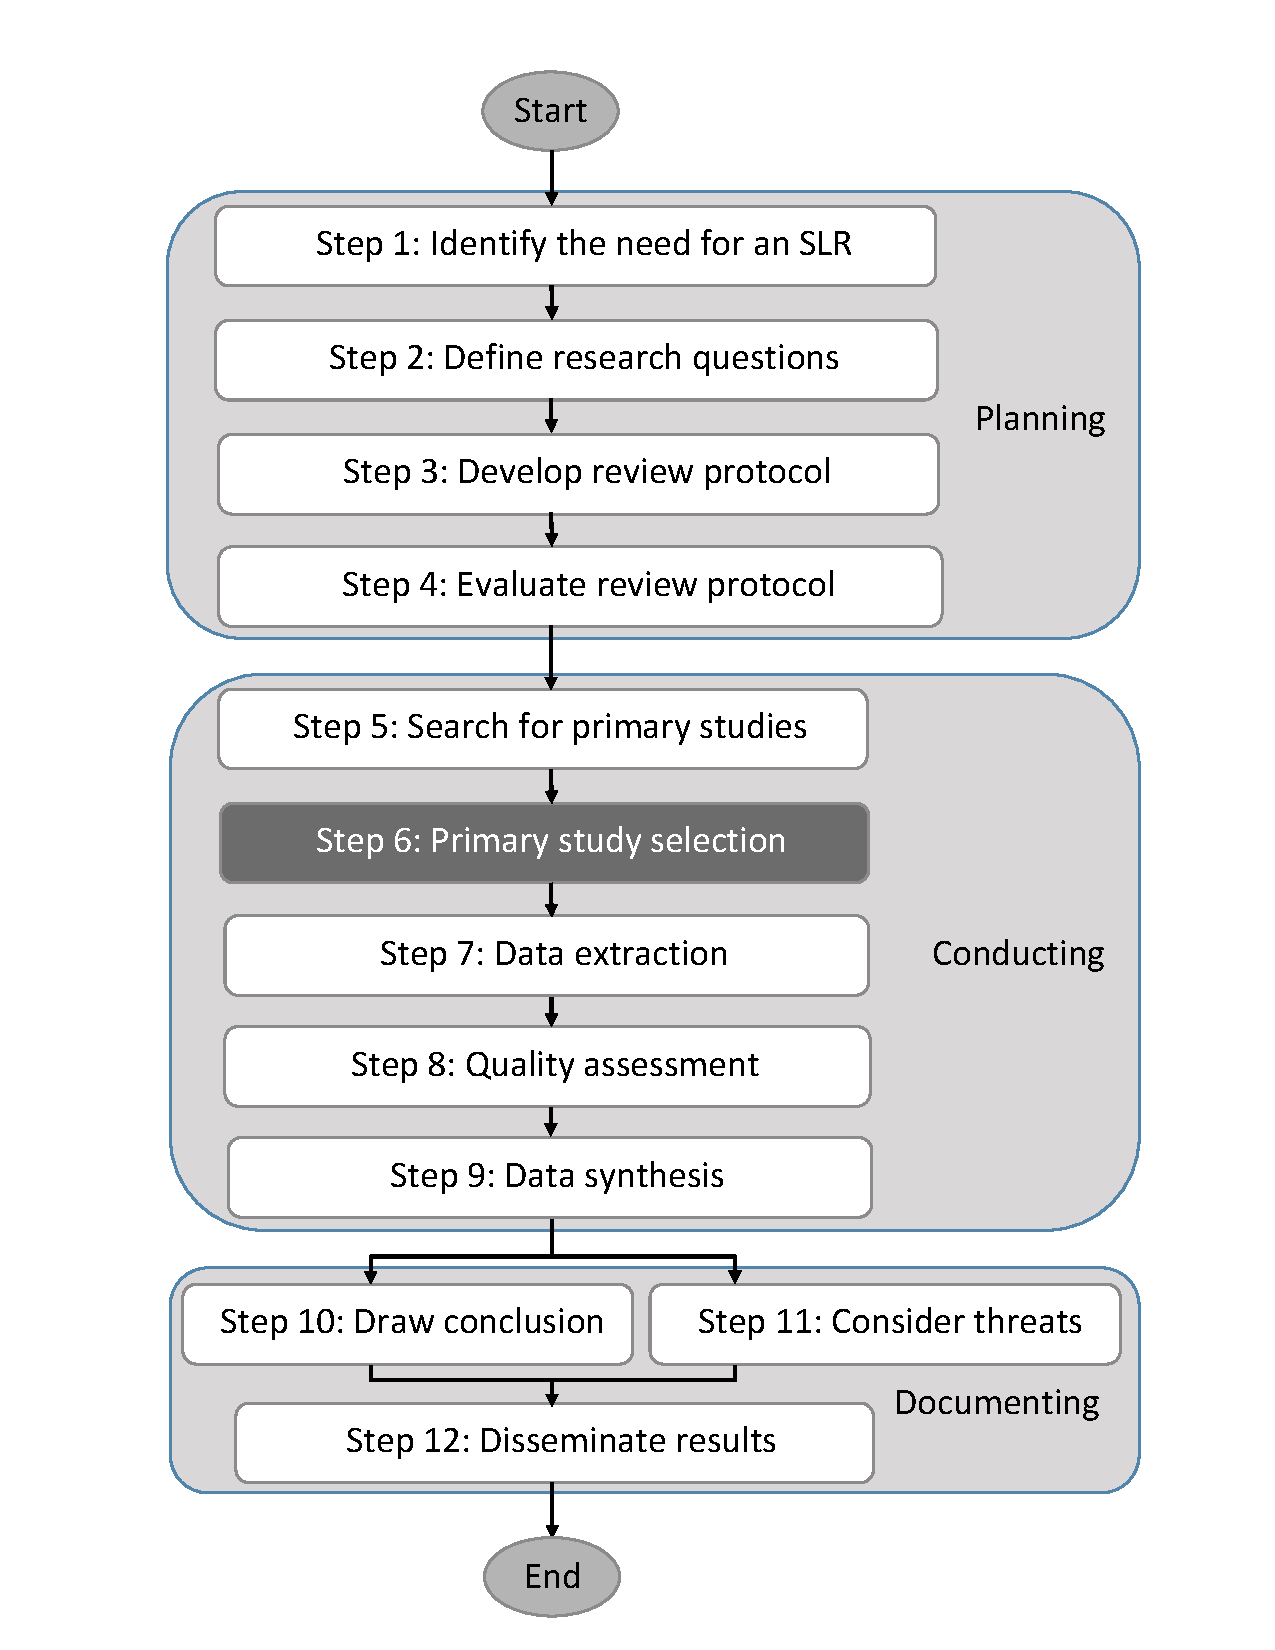
\includegraphics[width=\linewidth]{procedure.pdf}
    \caption{Systematic literature review steps suggested by \cite{keele2007guidelines}.}
    \label{fig: slr}
\end{figure}

In contrast to a primary study, which investigates a specific research question,
a systematic literature review is a form of secondary study aimed at
identifying, evaluating and interpreting all available research relevant to a
particular research question, topic area, or phenomenon of
interest~\cite{keele2007guidelines}. In the modern academic world, it is
impossible to start a research without first knowing what other researchers have
done in the topic area. Conducting an SLR is one way to gain
background knowledge on a certain topic area.
If that SLR is published, then that paper becomes a useful research tool
for other researchers.  Kitchenham recommend SLRs to be standard
procedure in SE research~\cite{kitchenham2004evidence,keele2007guidelines}.

An SLR is usually conducted following the procedures in Figure~\ref{fig:
  slr}. There can be variances on the real
implementations~\cite{wahono2015systematic,malhotra2015systematic,radjenovic2013software,unterkalmsteiner2012evaluation,hall2012systematic},
but all are based on the same guideline~\cite{keele2007guidelines}. In this
study, we focus on Step 6: primary study selection.

\ \\ \noindent
{\bf RQ1: What are the costs of a standard SLR primary study selection?} 

\subsection{Primary Study Selection}
\label{subsect: Primary Study Selection}

\begin{figure}[ht]
    \centering
    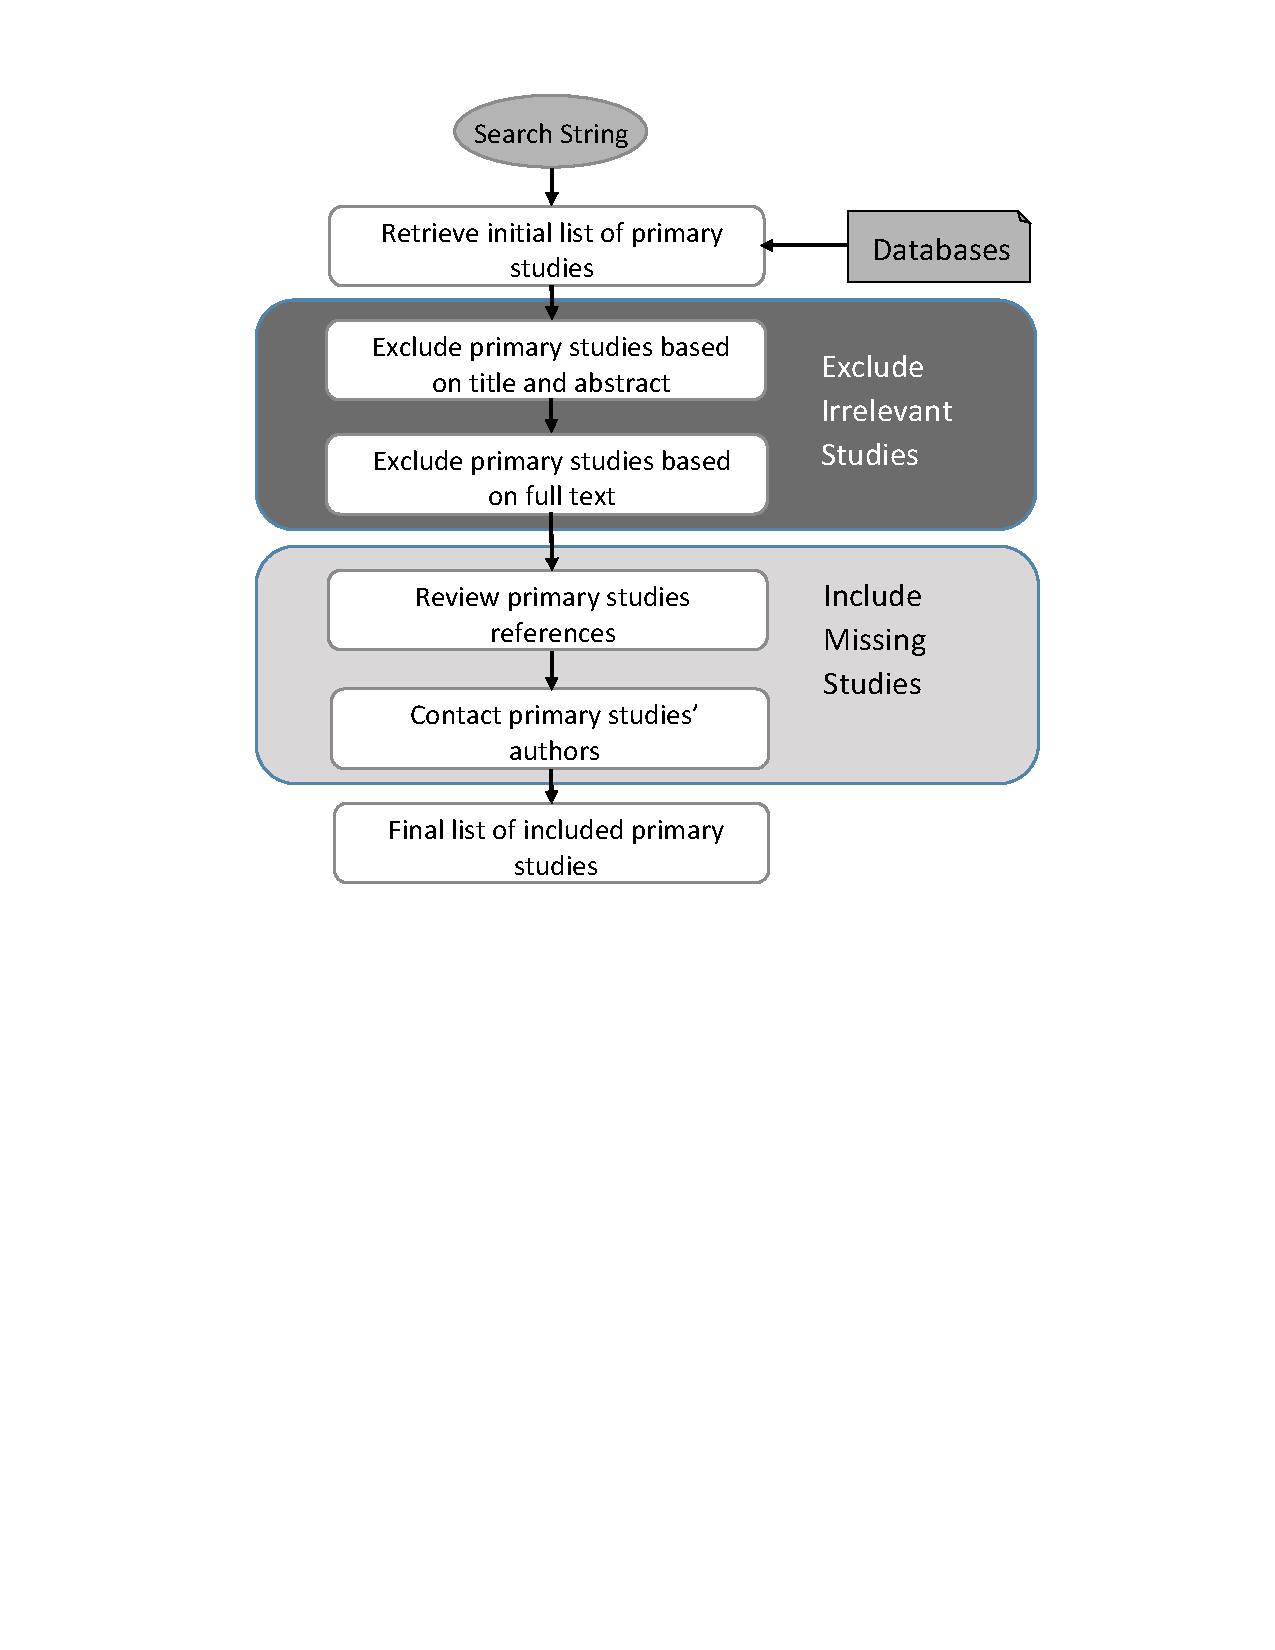
\includegraphics[width=\linewidth]{primary_study_selection.pdf}
    \caption{Primary study selection steps suggested by \cite{keele2007guidelines}.}
    \label{fig: prime}
\end{figure}

Primary study selection starts with an initial candidate collection of studies retrieved by searching. In the first round of that process,
the reviewers' job is to read the titles and abstracts of candidate studies and classify each as ``relevant'' or ``irrelevant''. After the first round of review, the reviewers read through the full text of the previously included studies and make further decision on whether it is actually ``relevant'' or not. The whole procedure is shown in Figure~\ref{fig: prime}. In this study, we focus on how to utilize machine learning algorithms to speed up the ``Exclude Irrelevant Studies'' step.

Typically, reviewers need to identify a final list of dozens of primary studies
among the initial collection of thousands of candidates. In terms of actual
cost, Malheiros has documented in \cite{malheiros2007visual} that it requires 3
hours for one reviewer to review 100 studies.  This implies that it is a month's
work for one graduate student to review 3000 studies or three month's work to
review 9000 studies. Also, in our previous studies, primary
study selection has been identified as one of the top three most time-consuming
and difficult step in SLR~\cite{carver2013identifying}, as well as one of the
top desired features to be automated by tools and has not yet been
supported~\cite{hassler2014outcomes,hassler2016identification,marshall2015tools,marshall2014tools}.


The target of this paper is to reduce the cost of the primary study selection by applying machine learning techniques to assist the review process since:

\begin{lesson}
    A major cost in SLR is the effort associated with primary study selection. Months of tedious work are required to review thousands of candidate studies.
\end{lesson}



\subsection{Related Works in Software Engineering}

In recent years, various tools have been developed to facilitate SLRs in software engineering community, as summarized in~\cite{marshall2015tools,marshall2014tools,marshall2013tools}. These tools aim at providing support for protocol development~\cite{Molleri:2015:SWA:2745802.2745825,fernandez2010slr,hernandes2012using}, automated search~\cite{Molleri:2015:SWA:2745802.2745825,hernandes2012using}, primary study selection~\cite{Molleri:2015:SWA:2745802.2745825,hernandes2012using,fernandez2010slr,bowes2012slurp}, quality assessment~\cite{fernandez2010slr,bowes2012slurp,Molleri:2015:SWA:2745802.2745825}, data extraction and validation~\cite{Molleri:2015:SWA:2745802.2745825,hernandes2012using,fernandez2010slr,bowes2012slurp}, data synthesis~\cite{Molleri:2015:SWA:2745802.2745825,hernandes2012using,fernandez2010slr,bowes2012slurp},
and report write up~\cite{Molleri:2015:SWA:2745802.2745825,hernandes2012using,fernandez2010slr,bowes2012slurp}. It is extremely helpful to have a tool for managing the whole SLR process. However, the support for primary study selection using these tools is limited (e.g., to tasks such as assigning review jobs to multiple reviewers or to resolving disagreements).
Hence, we assert that the current SE SLR literature provides
no tool that can offer reductions in the effort required for primary study selection comparable to those reductions offered by machine assisted reading. 

Visual text mining (VTM) is a technique especially explored in Software Engineering community to support SLR. It is an unsupervised learning method which visualizes the relationship between candidate studies and helps the reviewer to make quick decisions. Malheiros et al.~\cite{malheiros2007visual} first applied VTM to support primary study selection in SLR. In their small-scale experiment (100 candidate studies, 31 of which are ``relevant''), VTM retrieves around 90\% of the ``relevant'' studies by spending about 30\% as much time as manual review. However, VTM requires some prior experience and knowledge of text mining and visualization techniques to use~\cite{bowes2012slurp}, and more case studies with large scale are needed to validate their results. After the study of ~\cite{malheiros2007visual}, instead of being applied to assist primary study selection, VTM has been further explored to support systematic mapping~\cite{felizardo2010approach}, validate the primary study selection result~\cite{felizardo2012visual}, and the continuing update of SLR~\cite{Felizardo:2014:VAA:2601248.2601252}. VTM has thus been proved to be a powerful technique to help user better understand the hidden relationship between selected primary studies.

In this paper, we are exploring a different direction to reduce cost in primary
study selection. Instead of an unsupervised learning technique such as VTM, we use semi-supervised
learning method. Given the performance of our method --- i.e.,  90\% of the ``relevant''
studies can be found by reviewing only 10\% of the candidate studies --- we suggest that SLR
authors use our method for primary study selection but also use
tools like VTM before
and after the selection process to have a better understanding of the
studies. The potential of combining VTM and machine assisted reading to further
boost primary study selection is also considered in our future research.

Our work is the first to explore machine-assisted-reading for primary study selection in the software engineering community~\cite{hassler2016identification}.
However, other recent studies do focus on the search process for systematic literature reviews.
Zhang et al.~\cite{zhang2011empirical} assessed the QGS-based systematic search process for SLRs and found that use of such a search process can help both to identify more relevant studies and to save the time spent in the search process.
Jalali and Wohlin~\cite{jalali2012systematic} compared the use of two different search approaches --- database search and backward snowballing --- as the first step in the search process for SE SLRs and found that neither approach is the superior choice for the first step in the search process.

\ \\ \noindent 
{\bf RQ2: What are the state-of-the-art machine assisted reading techniques?} 

\subsection{Related Works in Evidence-based Medicine}
\label{sect: Evidence-based Medicine}

Systematic literature reviews were first adopted from evidence-based medicine in
2004~\cite{kitchenham2004evidence}. To facilitate citation screening (primary
study selection) in systematic review, Wallace conducted a series of studies
with machine learning techniques, especially active
learning~\cite{wallace2010semi,wallace2010active,wallace2011should,wallace2012deploying,wallace2013active,wallace2013modernizing,nguyen2015combining}. Wallace
first set up a baseline approach called ``patient active learning'', which will be explained later in this subsection, for machine learning assisted citation
screening~\cite{wallace2010semi}. The performance of patient active learning
is good enough (nearly 100\% of the ``relevant''
citations can be retrieved at half of the conventional review cost) to convince
systematic review conductors to adopt machine learning assisted citation
screening. Instead of improving this baseline method, Wallace then focused on other aspects of machine learning assisted citation screening such as introducing external expert knowledge~\cite{wallace2010active}, allocating review tasks to multiple experts~\cite{wallace2011should} or to crowd sourcing workers~\cite{nguyen2015combining}, and building a tool called abstrackr to provide overall support~\cite{wallace2012deploying}. 

Wallace's work on this topic is of  
exemplary high-impact and
 his core algorithm   (on simple expert screening),   is   the most
popular machine assisted reading technique we have found in the
evidence-based medical literature. That said,
this technique has not been updated   since 2010~\cite{wallace2010semi}.

In this paper we are focused on cost minimization. Hence, we do not explore
techniques such as Wallace's use of multiple experts (but in future work,
we will explore this approach).

Other work related to machine learning assisted citation screening do not
utilize active learning and machine assisted reading. Pure supervised learning
requires a sufficiently large training set, which leads to a huge review
cost~\cite{cohen2006reducing, adeva2014automatic}. Therefore the patient active
learning proposed by Wallace et al. is still the state-of-the-art method for
citation screening in the scenario with no external knowledge and equally
expensive reviewers. Details on patient active learning will be provided in Section~\ref{sect: Patient Active Learning}.



\subsection{Related Works in Electronic Discovery}
\label{sect: Electronic Discovery}

Electronic Discovery (e-discovery) is a part of civil litigation where one party (the producing party), offers up materials which are pertinent to a legal case~\cite{krishna2016bigse}. This involves a review task where the producing party need to retrieve every ``relevant'' document in their possession and turn them over to the requesting party. It is extremely important to reduce the review cost in e-discovery since in a common case, the producing party will need to retrieve thousands   of ``relevant'' documents among millions of candidates. Technology-assisted review (TAR) is the technique to facilitate the review process. The objective of TAR is to find as many
of the ``relevant'' documents in a collection as possible, with reasonable cost~\cite{grossman2013}. 

Interestingly, the relationship between e-discovery and evidence-based medicine have been discussed in~\cite{leasesystematic} but their methods are still diverged. Relying on Grossman and Cormack~\cite{grossman2013} for support, many legal service providers have adopted TAR to facilitate the review process.
The machine assisted reading methods applied in TAR are simple passive learning, simple active learning, and continuous active learning. So far, in every controlled studies, continuous active learning has outperformed others~\cite{cormack2014evaluation,cormack2015autonomy}, which makes it the state-of-the-art method in TAR. Details on continuous active learning will be provided in Section~\ref{sect: Continuous Active Learning}.



In summary: 
\begin{lesson}
    The state-of-the-art machine assisted reading techniques are patient active learning in evidence-based medicine and continuous active learning in e-discovery.
\end{lesson}








\section{Technical Briefing}
\label{sect: Technical Briefing}

\begin{figure}[!b]
    \centering
    \subfigure[Training SVM without data balancing]
    {
        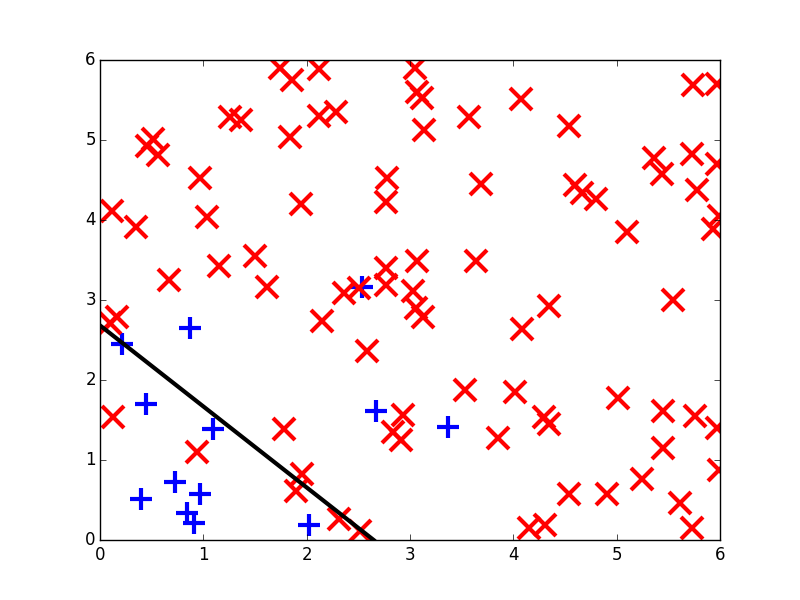
\includegraphics[width=0.46\linewidth]{train.png}
        \label{fig:train}
    }
    \subfigure[Training SVM with aggressive undersampling]
    {
        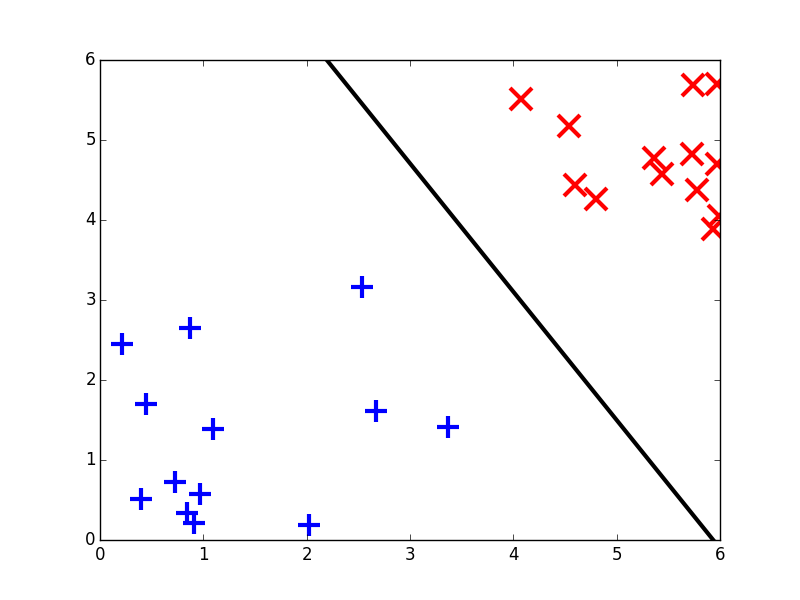
\includegraphics[width=0.46\linewidth]{train_a.png}
        \label{fig:train_a}
    }
    \quad
    \subfigure[Predictions with model in (a)]
    {
        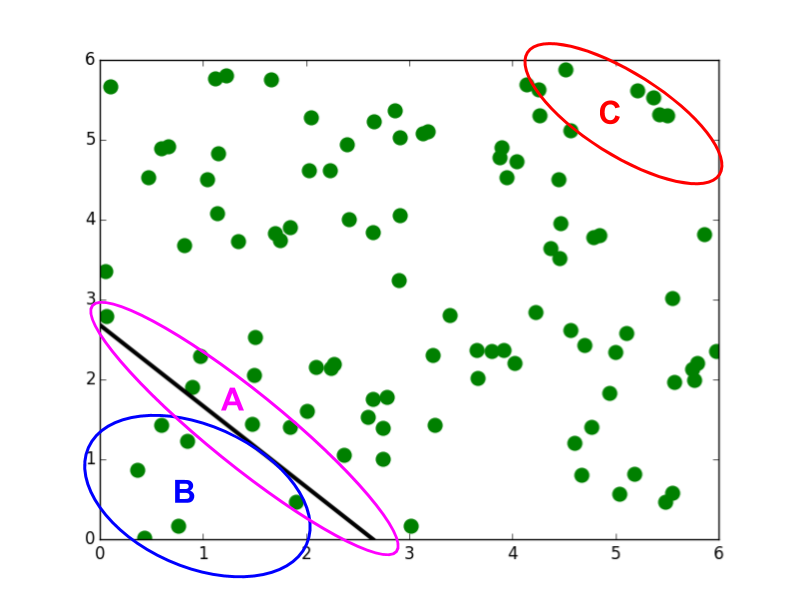
\includegraphics[width=0.46\linewidth]{test.png}
        \label{fig:test}
    }
    \subfigure[Predictions with model in (b)]
    {
        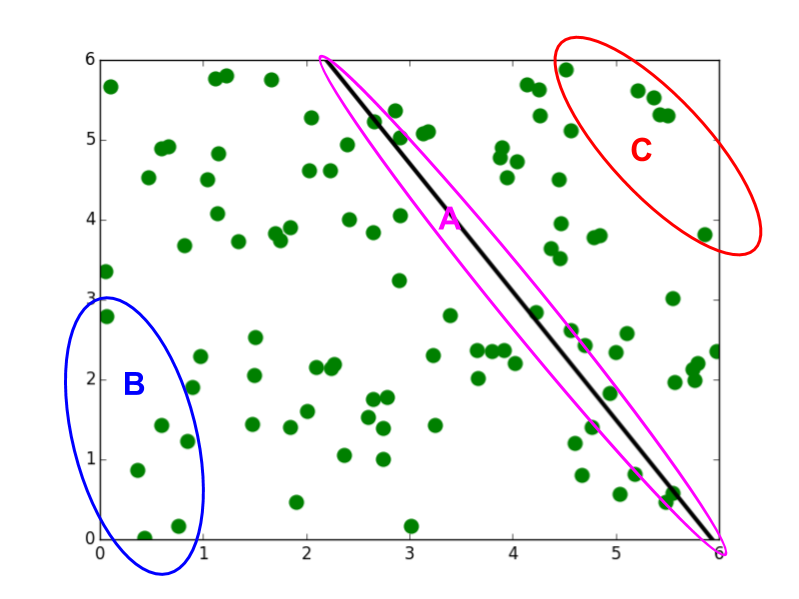
\includegraphics[width=0.46\linewidth]{test_a.png}
        \label{fig:test_a}
    }
    
    \caption{(a) and (b) shows how SVM model is trained on imbalanced data, where ``$+$'' is the minority class, ``relevant'' studies in SLR, ``$X$'' is the majority class, ``irrelevant'' studies in SLR, and black line is SVM decision plane. In (b), aggressive undersampling balances the training data by throwing away majority class examples closest to the old decision plane in (a). (c) and (d) show how SVM suggests the next batch of studies to be reviewed. In uncertainty sampling, Group A will be suggested since it is believed that the examples closest to the decision plane are most informative and once labeled, can help in training SVM most~\cite{settles2012active}. In certainty sampling, Group B will be suggested since they are of highest prediction probability of belonging to the relevant class ``$+$''.}
    \label{fig:SVM}
\end{figure}

In this section, we provide details on technical terms 
used in the paper,  along with some brief introductory
notes on machine learning techniques used in machine assisted reading.

\subsection{Support Vector Machine}
\label{sect: Support Vector Machine}

Support vector machine (SVM) is a well-known and widely used classification method. The idea behind is to map input data to a high-dimension feature space and then construct a linear decision plane in that feature space~\cite{cortes1995support}. Linear SVM~\cite{joachims2006training} has been proved to be a useful model in SE text mining~\cite{krishna2016bigse} and is applied in the state-of-the-art machine assisted reading methods of both evidence-based medicine and electronic discovery~\cite{wallace2010semi,cormack2014evaluation}. Figure~\ref{fig:SVM} illustrates linear SVM model on a two-dimension feature space.

\subsection{Active Learning}
\label{sect: Active learning}

Active learning is a cost-aware machine learning algorithm where labels of training data can be acquired with certain costs. The key idea behind active learning is that a machine learning algorithm can perform better with less
training if it is allowed to choose the data from which it learns~\cite{settles2012active}. There are several scenarios active learning is applied to, such as membership query synthesis, stream-based selective sampling, and pool-based sampling~\cite{settles2010active}. There are also different query strategies of active learning, such as uncertainty sampling, query-by-committee, expected model change, expected error reduction, variance reduction, and density-weighted methods~\cite{settles2010active}. Here, we will briefly introduce one scenario and two query strategies, which will be used in our later experiments and discussions.

\textbf{Pool-based sampling} is the scenario of primary study selection. This scenario starts with a fixed size pool of unlabeled data. Labels for the data can be acquired by querying an oracle selectively. The goal of pool-based sampling is to select the most informative data in the pool for query, thereby building a better model with less training.

\textbf{Uncertainty sampling} is the query strategy utilized in the state-of-the-art machine assisted reading technique of evidence-based medicine~\cite{wallace2010semi,wallace2010active}. It is also recognized as the most simple and commonly used query strategy~\cite{settles2010active}. In this query strategy, uncertainty sampling queries the instances about which the learner is least certain how to label. These instances are those (a) whose posterior probability of being positive are nearest 0.5 in probabilistic models or (b) closest to the decision boundary in models such as SVM. A demonstration of certainty sampling with SVM model can be found in Figure~\ref{fig:SVM}.

\textbf{Certainty sampling} is another query strategy which is applied in the state-of-the-art machine assisted reading technique of electronic discovery~\cite{cormack2014evaluation,cormack2015autonomy}. In contrast to uncertainty sampling, certainty sampling queries the instances about which the learner is most certain to label as positive. These instances are those (a) whose posterior probability of being positive are highest in probabilistic models, or (b) lies in the positive side of the decision boundary and furthest to the decision boundary in models such as SVM. A demonstration of certainty sampling with SVM model can be found in Figure~\ref{fig:SVM}. This query strategy is usually NOT used when building the classifier of active learning since it is commonly believed that examples queried by certainty sampling contains less information than those by uncertainty sampling.

\subsection{Machine assisted Reading}
\label{sect: Machine assisted Reading}

Machine assisted reading is a combination of manual review and machine
suggestions~\cite{tredennick2015}. In this approach:
\begin{itemize}
\item
Humans read a stream of documents, commenting on whether or
not each one is ``relevant''.
\item
  Machine learners use feedback from the human opinion to
  incrementally update their models actively.
\item
  The models generated via machine learning are used
  to sort the stream of documents such that the humans focus on the
  most informative documents.
  \end{itemize}

Machine assisted reading is a
pool-based active learning scenario since (1) the process starts with a fixed size candidate list without any labels and (2) training examples gradually become available to the learner as the human reviewer reviews the documents.  However, a significant difference between machine assisted reading and other active learning methods is that every document labeled as ``relevant'' has been reviewed by a human. The machine never makes the final decision on whether a document is ``relevant''; a human makes such decisions and the machine only suggests a review order based on the human's input. As a result, instead of building a better classification model, the objective of machine assisted reading is to retrieve most ``relevant'' documents from a pool of candidates while manually reviewing as few documents as possible. 

Simple active learning, which is pool-based active learning with uncertainty sampling~\cite{settles2012active}, is the most basic form of learning methods
applied to machine assisted reading. Although simple active learning achieves
satisfactory performance, it has been outperformed by the state-of-the-art machine assisted reading techniques in both evidence-based medicine~\cite{wallace2010semi} and electronic discovery~\cite{cormack2014evaluation}. 

\subsection{Patient Active Learning}
\label{sect: Patient Active Learning}

The state-of-the-art machine assisted reading method in evidence-based medicine, patient active learning can be described as following~\cite{wallace2010semi}:

\begin{itemize}

\item
{\bf Stage I: Construct an initial seed training set} by random sampling from the candidate study pool and asking a human reviewer to label the papers in the set as ``relevant'' or ``irrelevant''. Stop and proceed to Stage II when \textit{enough} ``relevant'' studies have been retrieved to represent the ``relevant'' class. (Note that Wallace et al.~\cite{wallace2010semi} do not provide an explicit definition of \textit{``enough''}.)

\item
{\bf Stage II: Build the classifier}, which is a linear SVM, by repeatedly training on labeled studies and uncertainty sampling. Unlabeled studies in the pool will be ranked in the descending order of uncertainty (uncertainty sampling). The human reviewer labels the studies in the ranked order and feeds them back to retrain the classifier. Stop and proceed to Stage III when the classifier is \textit{stable}. (Note that Wallace et al.~\cite{wallace2010semi} do not provide an explicit definition of \textit{``stable''}.)

\item
{\bf Stage III: Prediction.} Retrain the classifier with aggressive undersampling and then stop training. Unlabeled studies in the pool will be ranked in the descending order of the classifier's prediction probability of being ``relevant'' (certainty sampling as discussed in Section~\ref{sect: Active learning}). The human reviewer labels the studies in the ranked order until finished (running out of review cost budget, enough ``relevant'' studies found, or no more ``relevant'' studies are detected in multiple rounds).

\end{itemize}

{\bf Aggressive undersampling: }The data for citation screening are (at times, extremely) imbalanced, i.e., the prevalence of ``relevant'' citations is always smaller than $50\%$ (and often much smaller). Classification algorithms are typically optimized for overall accuracy, rather than accuracy, precision, recall to a particular class. This becomes a problem when only the performance on a minority class matters. Patient active learning utilizes aggressive undersampling for data balancing. By throwing away majority (``irrelevant'') class training examples which are closest to the SVM decision hyperplane, it undersamples the majority class training examples to the same size as minority (``relevant'') class. It is a recall friendly undersampling method since the new decision hyperplane is pushed away from the minority class. An exampling of aggressive undersampling is shown in Figure~\ref{fig:SVM}.

\subsection{Continuous Active Learning}
\label{sect: Continuous Active Learning}

The state-of-the-art machine assisted reading method in e-discovery, continuous active learning can be described as following~\cite{cormack2014evaluation,cormack2015autonomy,tredennick2015}:

\begin{itemize}

\item
{\bf Stage I: Construct an initial seed training set} by random sampling from the candidate study pool and ask a human reviewer for labels. Stop and proceed to Stage II as soon as \textbf{ONE} ``relevant'' study is retrieved.

\item
{\bf Stage II: Predict and retrain} by repeatedly training on labeled studies and certainty sampling. Unlabeled studies in the pool will be ranked in the descending order of the classifier's prediction probability of being ``relevant'' (certainty sampling). A human reviewer labels the studies in the ranked order and feeds them back to retrain the classifier until finished.

\end{itemize}

In contrast to patient active learning, continuous active learning is the opposite of ``patient''. It starts to train the model as soon as \textit{ONE} ``relevant'' study shows up and skips the uncertainty sampling stage, which is believed to be essential for active learners~\cite{settles2012active}. The reason for this ``greedy'' strategy can be derived from the objective of machine assisted reading mentioned in Section~\ref{sect: Machine assisted Reading}. Since the objective is to retrieve ``relevant'' studies with candidates reviewed as few as possible, it is reasonable not to waste any single effort on building up the classifier~\cite{cormack2014evaluation,tredennick2015}. Also, the experiment results in \cite{cormack2014evaluation} has demonstrated the value of this ``greedy'' strategy.











\section{Methods}
\label{sect: Method}

This section describes our data sets and their preparation then describes and refactors state-of-the-art methods for machine assisted reading.
This refactoring process will create FASTREAD, our preferred machine assisted reading
method. 

\subsection{Data Sets}
\label{sect: Data Sets}

Although a large number of SLRs are published every year, there is no data set clearly documenting the details in primary study selection. As a result, two data sets are collected from existing SLRs and being used in this study\footnote{Available at \textit{https://doi.org/10.5281/zenodo.192506}}. The first data set is extracted from the SLR on defect prediction by Wahono in 2015~\cite{wahono2015systematic}. The second data set is extracted from the SLR on defect prediction by Hall and et al. in 2012~\cite{hall2012systematic}. 

For each of the data set, we retrieve the initial candidate collection from IEEE Xplore with the search string stated in the original literature. Then make a final list of inclusion by comparing the initial collection retrieved and the final list proposed in the corresponding SLR. Here, for simplicity reason we only extract candidate studies from single data source, IEEE Xplore. We will explore possibilities for efficiently utilizing multiple data sources in the future work but in this paper, without loss of generality, we only extract initial candidate list from single data source. 

The number of studies we retrieved from IEEE Xplore is listed in ``Retrieved'' columns of Table~\ref{tab: number}. On the other hand, in their original publications~\cite{wahono2015systematic,hall2012systematic}, the candidate primary studies are collected from multiple databases. The number of studies they retrieved is listed in ``Stated'' columns of Table~\ref{tab: number}.

\begin{table}
\caption{Descriptive statistics for experimental data sets}
\label{tab: number}
\begin{center}
\begin{tabular}{ |l|c|c|c|c| }
  \hline
   & \multicolumn{2}{|c|}{Wahono} & \multicolumn{2}{|c|}{Hall}\\
  \cline{2-5}
  & Stated & Retrieved & Stated & Retrieved\\
  \hline
  Initial list & 2117 & 7002 & 2073 & 8911\\
  \hline
  Final list & 72 & 62 & 136 & 106 \\
  \hline
\end{tabular}
\end{center}
\end{table}


In \cite{wahono2015systematic}, Wahono et al. applied the following search string
\begin{quote}\textit{(software OR applicati* OR systems ) AND (fault* OR
defect* OR quality OR error-prone) AND (predict*
OR prone* OR probability OR assess* OR detect* OR
estimat* OR classificat*)}
\end{quote}
to databases including IEEE Xplore, ACM Digital Library, ScienceDirect, Springer, and Scopus, to retrieve the initial candidate study set. After deduplication, an initial list of 2117 candidate studies are found. As a result of linearly review all 2117 studies, a final inclusion list of 71 studies are identified. On the other hand, we retrieve much more candidates with the same search string just from IEEE Xplore and cover about 85\% of the final list, as shown in Table~\ref{tab: number}. The final Wahono data set contains 7002 studies and 62 of which are labeled as ``relevant''.

In \cite{hall2012systematic}, Hall et al. applied the following search string
\begin{quote}{\em (Fault* OR bug* OR defect* OR errors OR corrections OR corrective OR fix*) \textit{in title only}
AND (Software) \textit{anywhere in study} }
\end{quote}
to databases including IEEE Xplore, ACM Digital Library, and ISI Web of Science, to retrieve the initial candidate study set. After deduplication, an initial list of 2073 candidate studies are found. As a result of linearly review all 2073 studies, a final inclusion list of 136 studies are identified. On the other hand, we again retrieve much more candidates with the same search string just from IEEE Xplore and cover about 75\% of the final list, as shown in Table~\ref{tab: number}. The final Hall data set contains 8911 studies and 106 of which are labeled as ``relevant''.

Although we have tried our best, the two data sets are still not exactly the same as described in the original studies~\cite{wahono2015systematic,hall2012systematic}. As shown in Table~\ref{tab: number}, the differences are from two aspects: 

\begin{itemize}

\item
More candidate studies are retrieved with the same search string than those in \cite{wahono2015systematic,hall2012systematic};

\item
Not all the ``relevant'' studies in the final inclusion lists of \cite{wahono2015systematic,hall2012systematic} are in our retrieved candidate study list.

\end{itemize}

The first difference is because, as stated in \cite{wahono2015systematic}, the search string is always refined manually in order to retrieve a satisfied candidate study list. This effort is always not exposed in SLRs and thus hinders our attempt to reproduce the candidate study list. This refinement of search string is actually a common attempt to reduce the size of candidate study list, thus save review effort in primary study selection with some sacrifice on completeness. With machine assisted primary study selection, the refinement of the search string is no longer necessary, because we can now tackle large candidate study list with a small amount of effort. Therefore, it is possible that the completeness will even increase when 90\% of ``relevant'' studies are retrieved, given that we now have a richer candidate list of studies.

The second difference is mainly because the candidate study lists are retrieved from IEEE Xplore only, while some of the ``relevant'' studies in the final inclusion lists of \cite{wahono2015systematic,hall2012systematic} are not in IEEE Xplore. It is for simplicity of the experiments since IEEE Xplore covers most of the studies. This may lead to a sampling bias between our experiment and real SLR process. However, we believe that our data sets are representative enough to compare different machine assisted reading methods in Section~\ref{sect: Algorithm Code}.

\subsection{Machine assisted Primary Study Selection}
\label{subsect: Learning based Primary Study Selection}


The general form of machine-assisted primary study selection is presented in
Figure~\ref{fig: learning}. Reviewers first review the title and abstract of the
suggested study, determine whether it is ``relevant'' or not. If the study is
``relevant'' by title and abstract, the reviewer will then read the full text of
the study and make the final decision. In the meantime, all the reviewed
studies, labeled as ``relevant'' or ``irrelevant'', will go into the training
set. Note that only the title and abstract of the training set studies will be used to
train the machine assisted reading model, thus making data extraction for training examples easy.

To simplify our analysis, as well as to facilitate comparison of different methods,
we make the following assumptions:

\begin{itemize}

\item
There is one single reviewer who never makes mistakes;

\item
The reviewer can access no external knowledge for building up initial seed training set;

\item
The goal is binary classification: studies will be labeled as ``relevant'' or ``irrelevant'' by the reviewer.

\end{itemize}
Note that, we are currently working on other scenarios where one or more of the
above assumptions are violated.  At this time we have nothing definitive to
report on those other scenarios. Hence, this rest of this paper will be in the context
of the above three assumptions.

As mentioned in Section~\ref{sect: Machine assisted Reading}, the objective of machine assisted primary study selection (or machine learning
assisted citation screening or TAR) is different from that of common active
learning scenario. In stead of trying to build a classifier as good as possible,
machine assisted primary study selection seeks methods to retrieve almost every
``relevant'' studies with candidate studies reviewed as few as possible. This
difference in the objective leads to a different performance metrics (further explained in Section~\ref{subsect: Performance Metrics}) and thus
makes conventional active learning methods being outperformed by specially
designed methods like patient active learning in evidence-based
medicine~\cite{wallace2010semi} and continuous active learning in
e-discovery~\cite{cormack2014evaluation,cormack2015autonomy}.


\begin{figure}[!t]
    \centering
    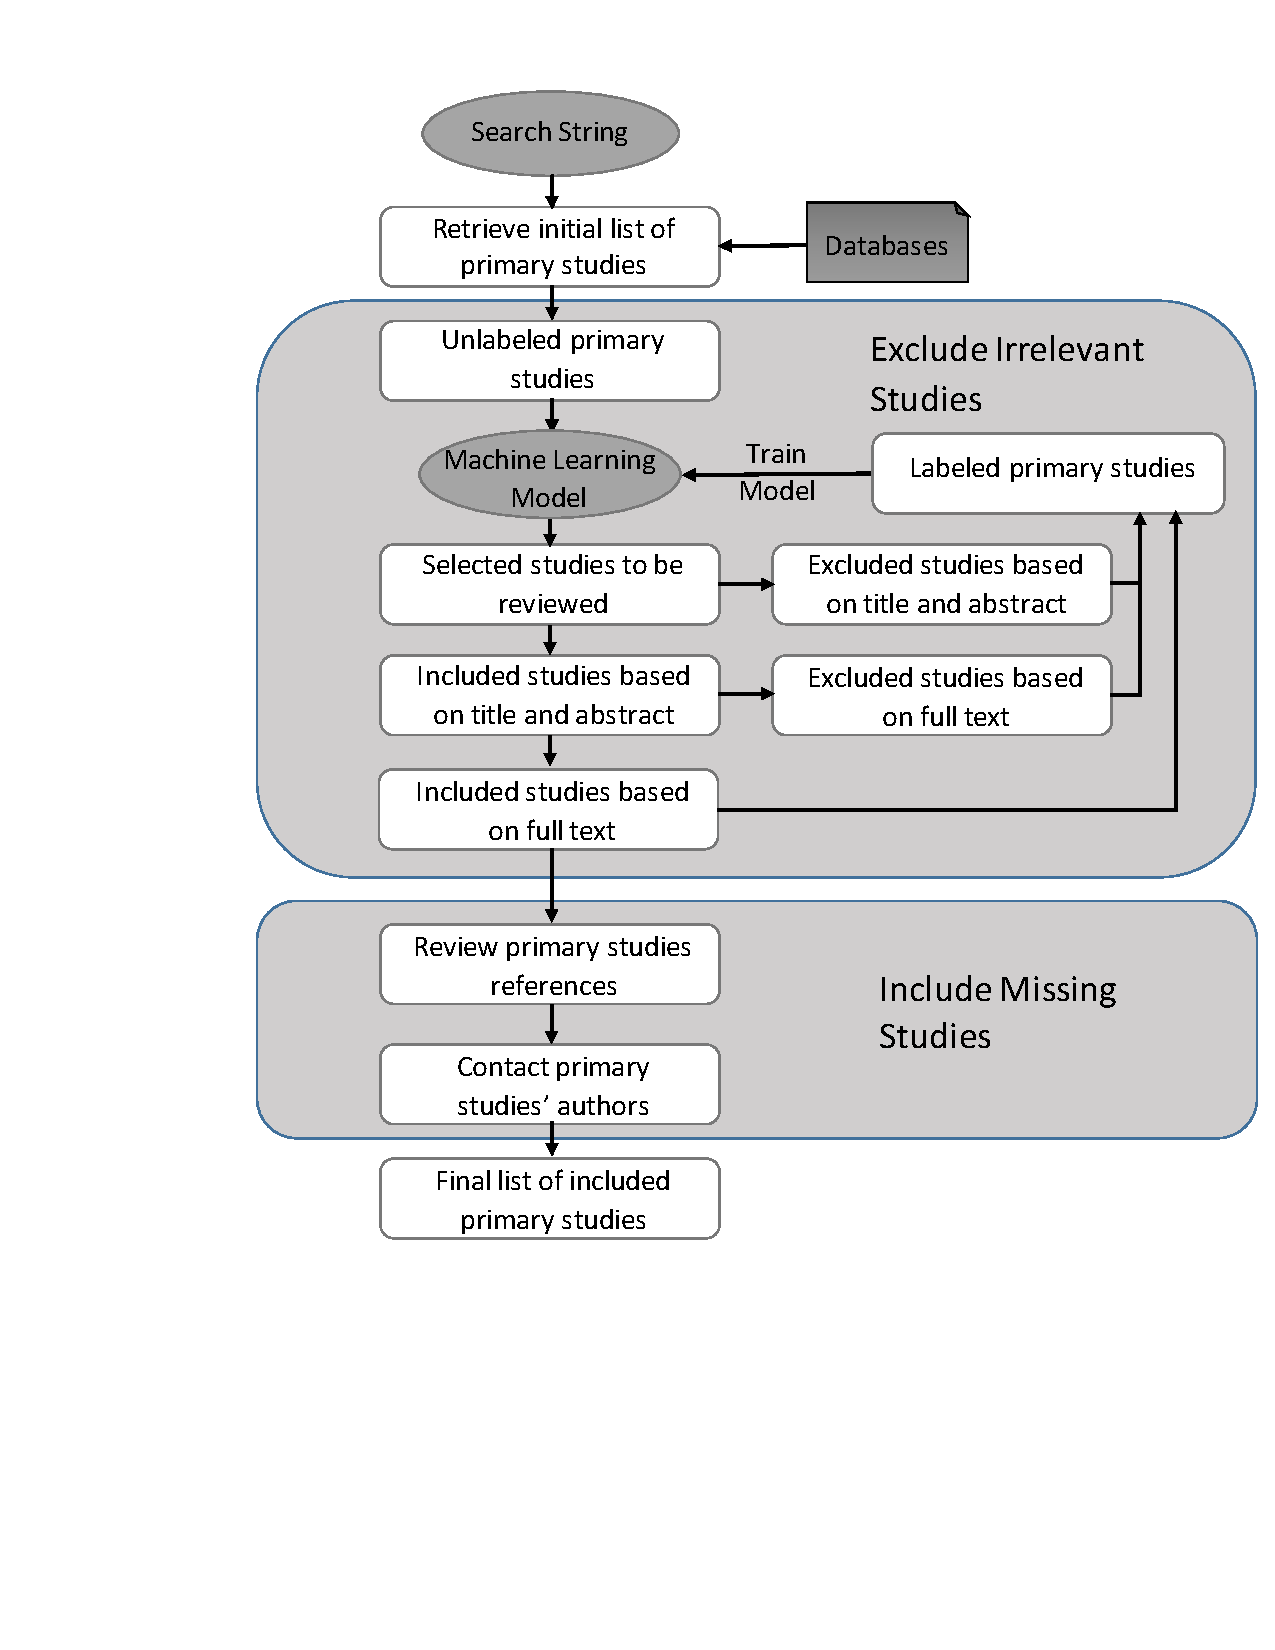
\includegraphics[width=\linewidth]{Learning_based_primary_study_selection.pdf}
    \caption{Machine assisted Primary study selection.}
    \label{fig: learning}
\end{figure}

\subsection{Algorithm Code}
\label{sect: Algorithm Code}

In order to utilize the advantages of both patient active learning and continuous active learning, we test and compare various of different combinations of the two algorithms in our experiments, Section~\ref{sect: Experiments}. The algorithms are coded following the principles below:

\begin{itemize}

\item
{\bf Code $P$}. 

\textbf{$P$} stands for ``patient''. The algorithm keeps random sampling until a sufficient number of ``relevant'' studies retrieved, as suggested in patient active learning. In our experiments, the sufficient number of ``relevant'' studies retrieved is set to $5$, which means when at least $5$ ``relevant'' studies have been retrieved by random sampling, the algorithm goes into next stage.

\textbf{$\bar{P}$} is the opposite. The algorithm stops random sampling as long as {\em ONE} ``relevant'' studies are retrieved, as suggested in continuous active learning.

\item
{\bf Code $U$}. 

\textbf{$U$} stands for ``uncertainty sampling''. The algorithm utilizes
uncertainty sampling to build the classifier, as suggested in patient active
learning. In our experiments, classifier is treated as ``stable'' once the margin
of SVM model is greater or equal to $2$. Uncertainty sampling stops once the
classifier is stable and goes into next step. Thereafter, certainty sampling
will start and the candidate studies with highest probability to be ``relevant''
will be returned. Figure~\ref{fig:test} and \ref{fig:test_a} shows the
difference between uncertainty sampling and certainty sampling where uncertainty
sampling returns Group A and certainty sampling returns Group B.

\textbf{$\bar{U}$} skips uncertainty sampling step and goes directly to certainty sampling with classifier retrained each round, as suggested in continuous active learning.

\item
{\bf Code $S$}. 

\textbf{$S$} stands for when to ``stop training''. The algorithm stops training
once the classifier is stable, as suggested in patient active learning.

\textbf{$\bar{S}$} stands for ``continuous learning''. The algorithm never stops
training as suggested in continuous active learning.

\item
{\bf Code $A$}. 

\textbf{$A$} stands for ``aggressive undersampling''. The algorithm utilizes aggressive undersampling when performing certainty sampling\footnote{We noticed that aggressive undersampling should not be performed with too few ``relevant'' training examples, as it only keeps twice the number of ``relevant'' training examples. Specifically, in $\bar{P}\bar{U}\bar{S}A$, certainty sampling with a classifier trained with only two examples leads to a huge deterioration in performance. Therefore we set a threshold for performing aggressive undersampling, i.e. not to begin aggressive undersampling until $M$ ``relevant'' studies have been retrieved, where $M=30$ in our experiment since a sample size of $30$ is usually
enough to approximate the distribution of each class~\cite{isotalo2001basics}.}, as suggested by patient active learning. Figure~\ref{fig:train_a} shows how an SVM is trained with aggressive undersampling and Figure~\ref{fig:test_a} shows how the prediction is affected.

\textbf{$\bar{A}$} stands for no data balancing. The algorithm does not apply any data balancing method when performing certainty sampling, as suggested by continuous active learning.

\end{itemize}

As a result, we ended up with 12 (\textbf{Code $\bar{U}$} and \textbf{Code $\bar{C}$} cannot coexist) algorithms including patient active learning as $PUSA$ and continuous active learning as $\bar{P}\bar{U}\bar{S}\bar{A}$. All the 12 algorithms are tested and compared in Section~\ref{sect: Experiments}.

\section{Experiments}
\label{sect: Experiments}

This section describes the experimental procedures that we used to evaluate the algorithms described in Section~\ref{subsect: Learning based Primary Study Selection} on the data sets described in Section~\ref{sect: Data Sets}

\subsection{Controlled Variables}
\label{subsect: Controlled Variables}

For the sake of a fair comparison, different algorithms in Section~\ref{sect: Algorithm Code} share an identical set of controlled variables including preprocessing and classifier. 

\subsubsection{Preprocessing}

\begin{figure}
    \centering
    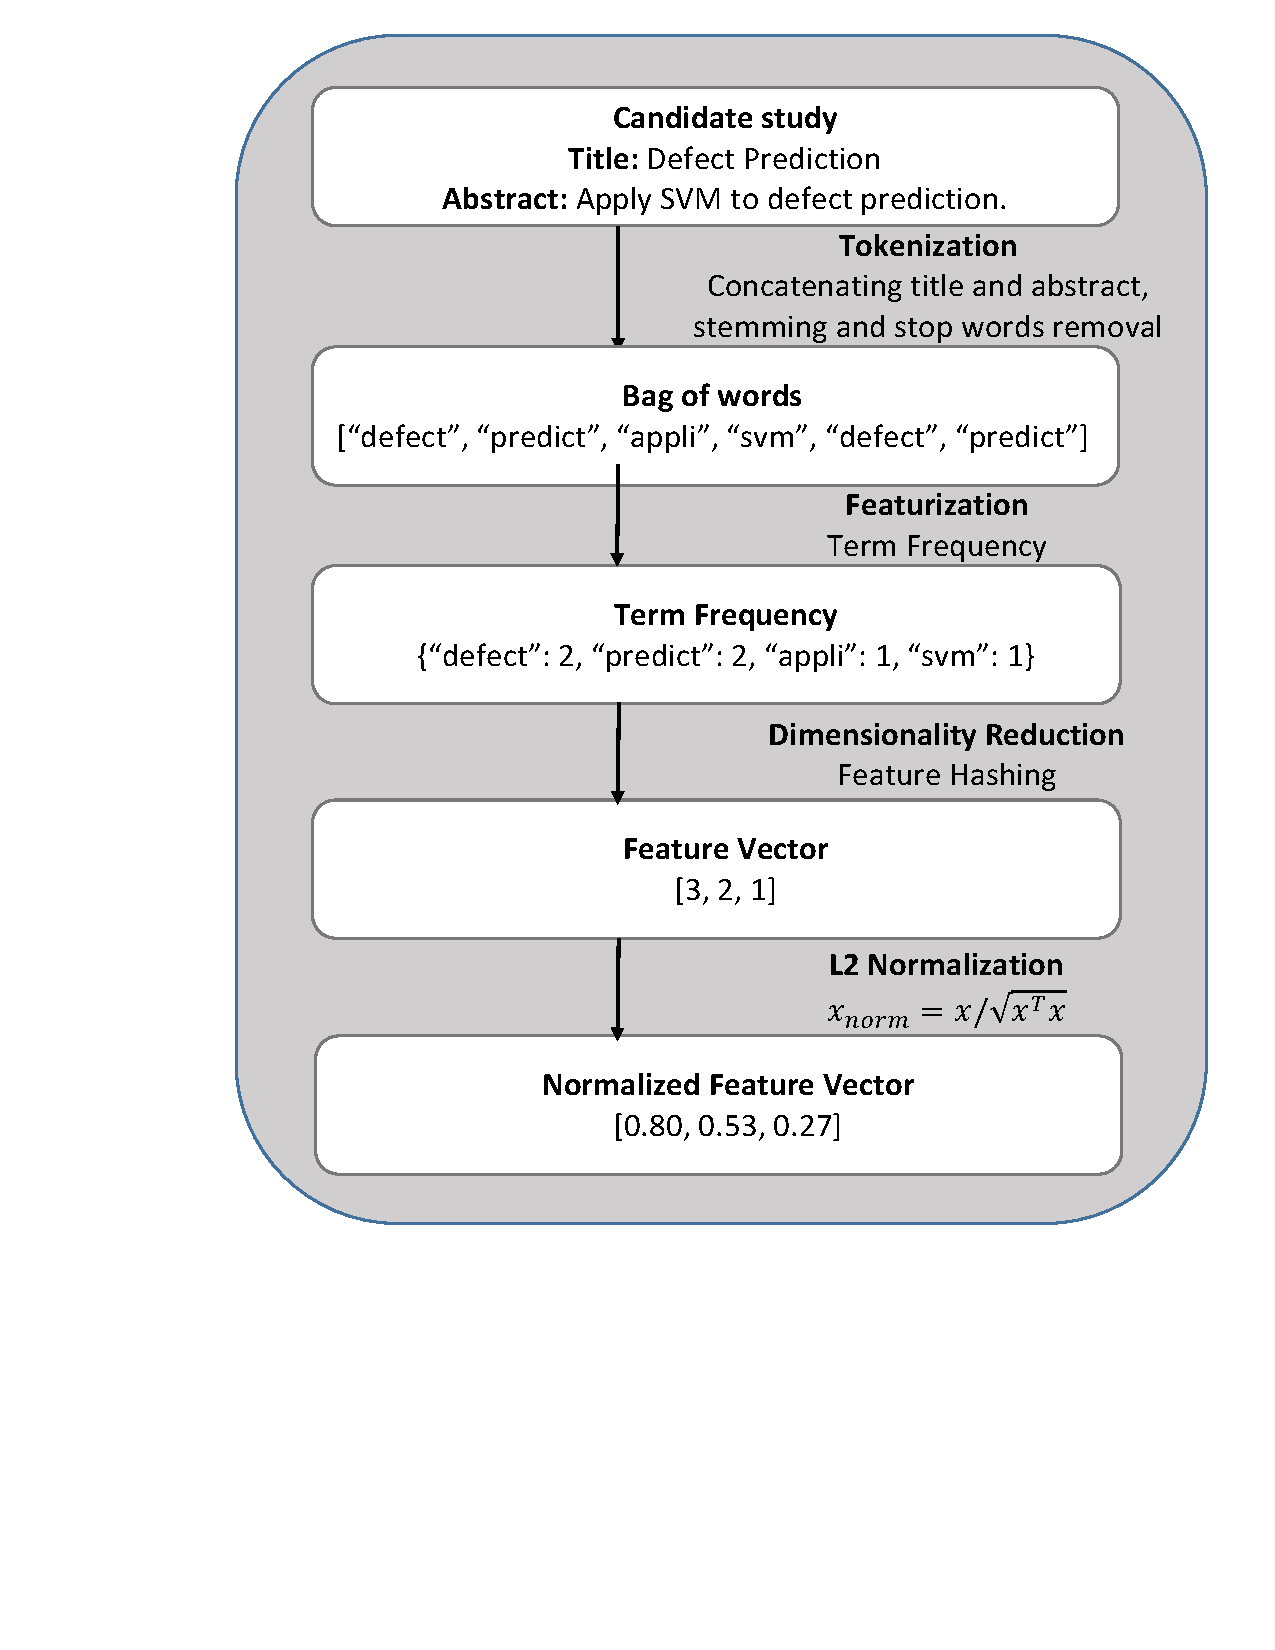
\includegraphics[width=\linewidth]{Preprocessing.pdf}
    \caption{Preprocessing process suggested by \cite{krishna2016bigse}.}
    \label{fig: preprocessing}
\end{figure}

Each candidate study in the initial list is first tokenized by stemming and stop words removal after concatenating its title and abstract. After tokenization, the bag of words are featurized into a term frequency vector. Then, reduce the dimensionality of the term frequency vector with feature hashing and normalize the hashed matrix by its L2 norm each row at last. The whole preprocessing process is presented in Figure~\ref{fig: preprocessing}. This preprocessing process is suggested and justified by~\cite{krishna2016bigse}.

\subsubsection{Classifier}

For this work we use a
linear SVM as the classifier.
SVMs learn a hyperplane that separate relevant from irrelevant examples
in the training data.
Linear SVMs do not make complicated assumptions about the data space
and so are known to scale to very large, high-dimensional
problems~\cite{joachims2006training}. Such linear SVMs are widely used in text
mining~\cite{krishna2016bigse}.
SVM's hyperplane is a natural tool for deciding what examples
to show next to the human user. As discussed in Section~\ref{sect: Technical Briefing}, uncertainty sampling prefers the examples
{\em closest} to the hyperplane boundary since these are the ones whose classification will
change, given small changes to the test data.
On the other hand, certainty sampling prefers
the examples {\em furthest} from this boundary since they are the ones that SVM is most certain about. 

\subsection{Performance Metrics}
\label{subsect: Performance Metrics}

Common active learning aims for building a better model with less training. Therefore its performance metrics is usually some \textbf{accuracy/precision/recall} on the model prediction vs \textbf{training size} curve. The \textbf{accuracy/precision/recall} are measured on some validation set.

On the other hand, since the goal of machine assisted primary study selection described in Section~\ref{subsect: Learning based Primary Study Selection} is different from that of common active learning, the performance metrics is also different. In machine assisted primary study selection, the performance of each algorithm is evaluated by its \textbf{recall} vs. \textbf{studies reviewed} curve. The \textbf{recall} here is not a measurement on the trained model, but the number of ``relevant'' studies retrieved over the total number of ``relevant'' studies. An algorithm is better than the other if it can retrieve more ``relevant'' studies with less studies reviewed, in other words, the upper left corner is the winning zone in this \textbf{recall} vs. \textbf{studies reviewed} curve. This performance metrics is suggested by \cite{cormack2015autonomy,cormack2014evaluation,tredennick2015} and best fits the objective of machine assisted primary study selection.

Each experiment repeats $30$ times\footnote{It is suggested that usually a sampling size of $30$ is adequate~\cite{isotalo2001basics}.}, the medians and different percentiles for every algorithm are collected and plotted on the graph. Every algorithm is compared by the corresponding values. A higher median in recall means the algorithm is able to retrieve more ``relevant'' studies with same amount of studies reviewed. The closer the results from different percentiles are, the less variance an algorithm has, thus more stable.


\subsection{Results}
\label{subsect: Results}



\begin{figure*}
    \centering
    \subfigure[Is FASTREAD better than state-of-the-art treatments?]
    {
        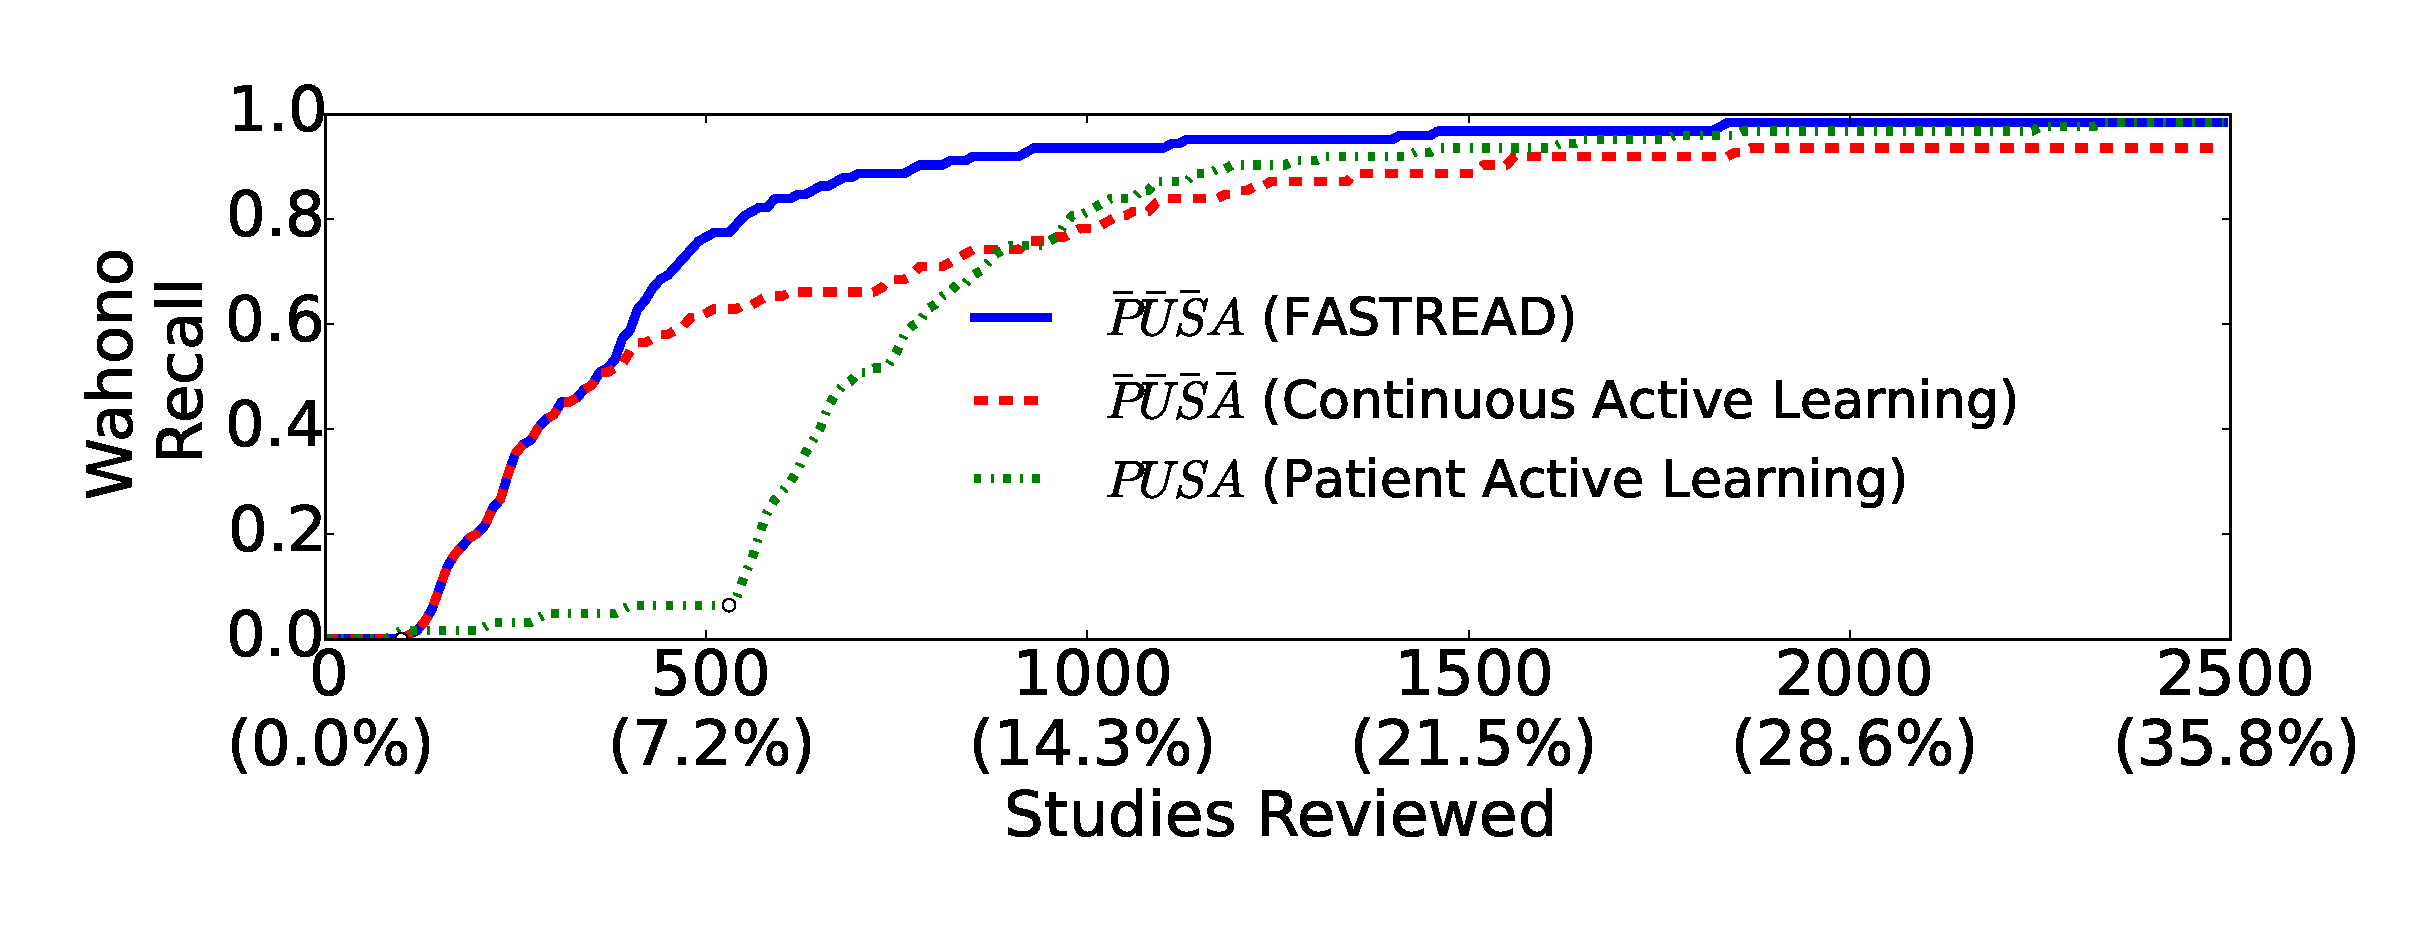
\includegraphics[width=0.48\linewidth]{IST_0_Wahono.eps}
        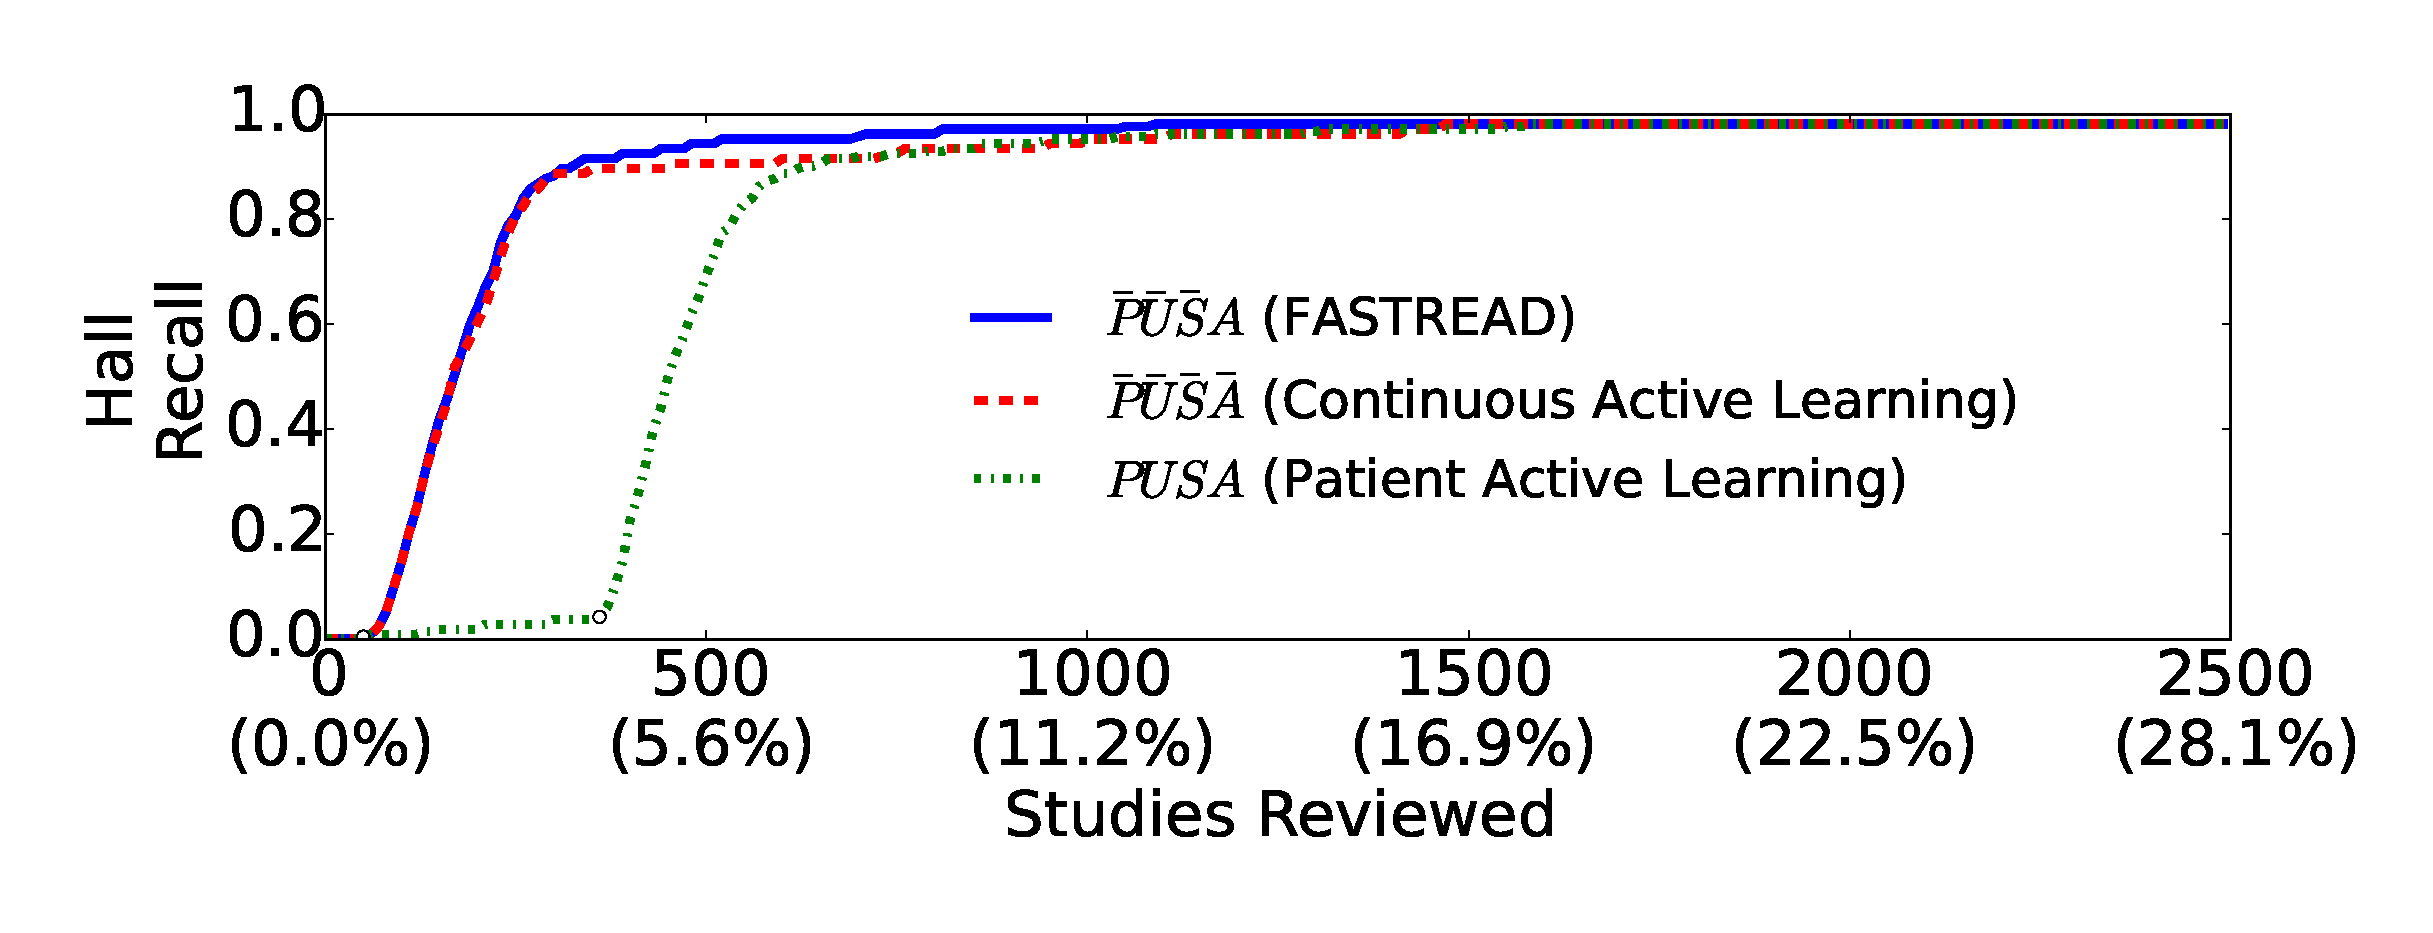
\includegraphics[width=0.48\linewidth]{IST_0_Hall.eps}
        \label{fig: baseline}
    }   
    \quad
    \subfigure[Is aggressive undersampling useful? Comparison for \textbf{Code A}.]
    {
        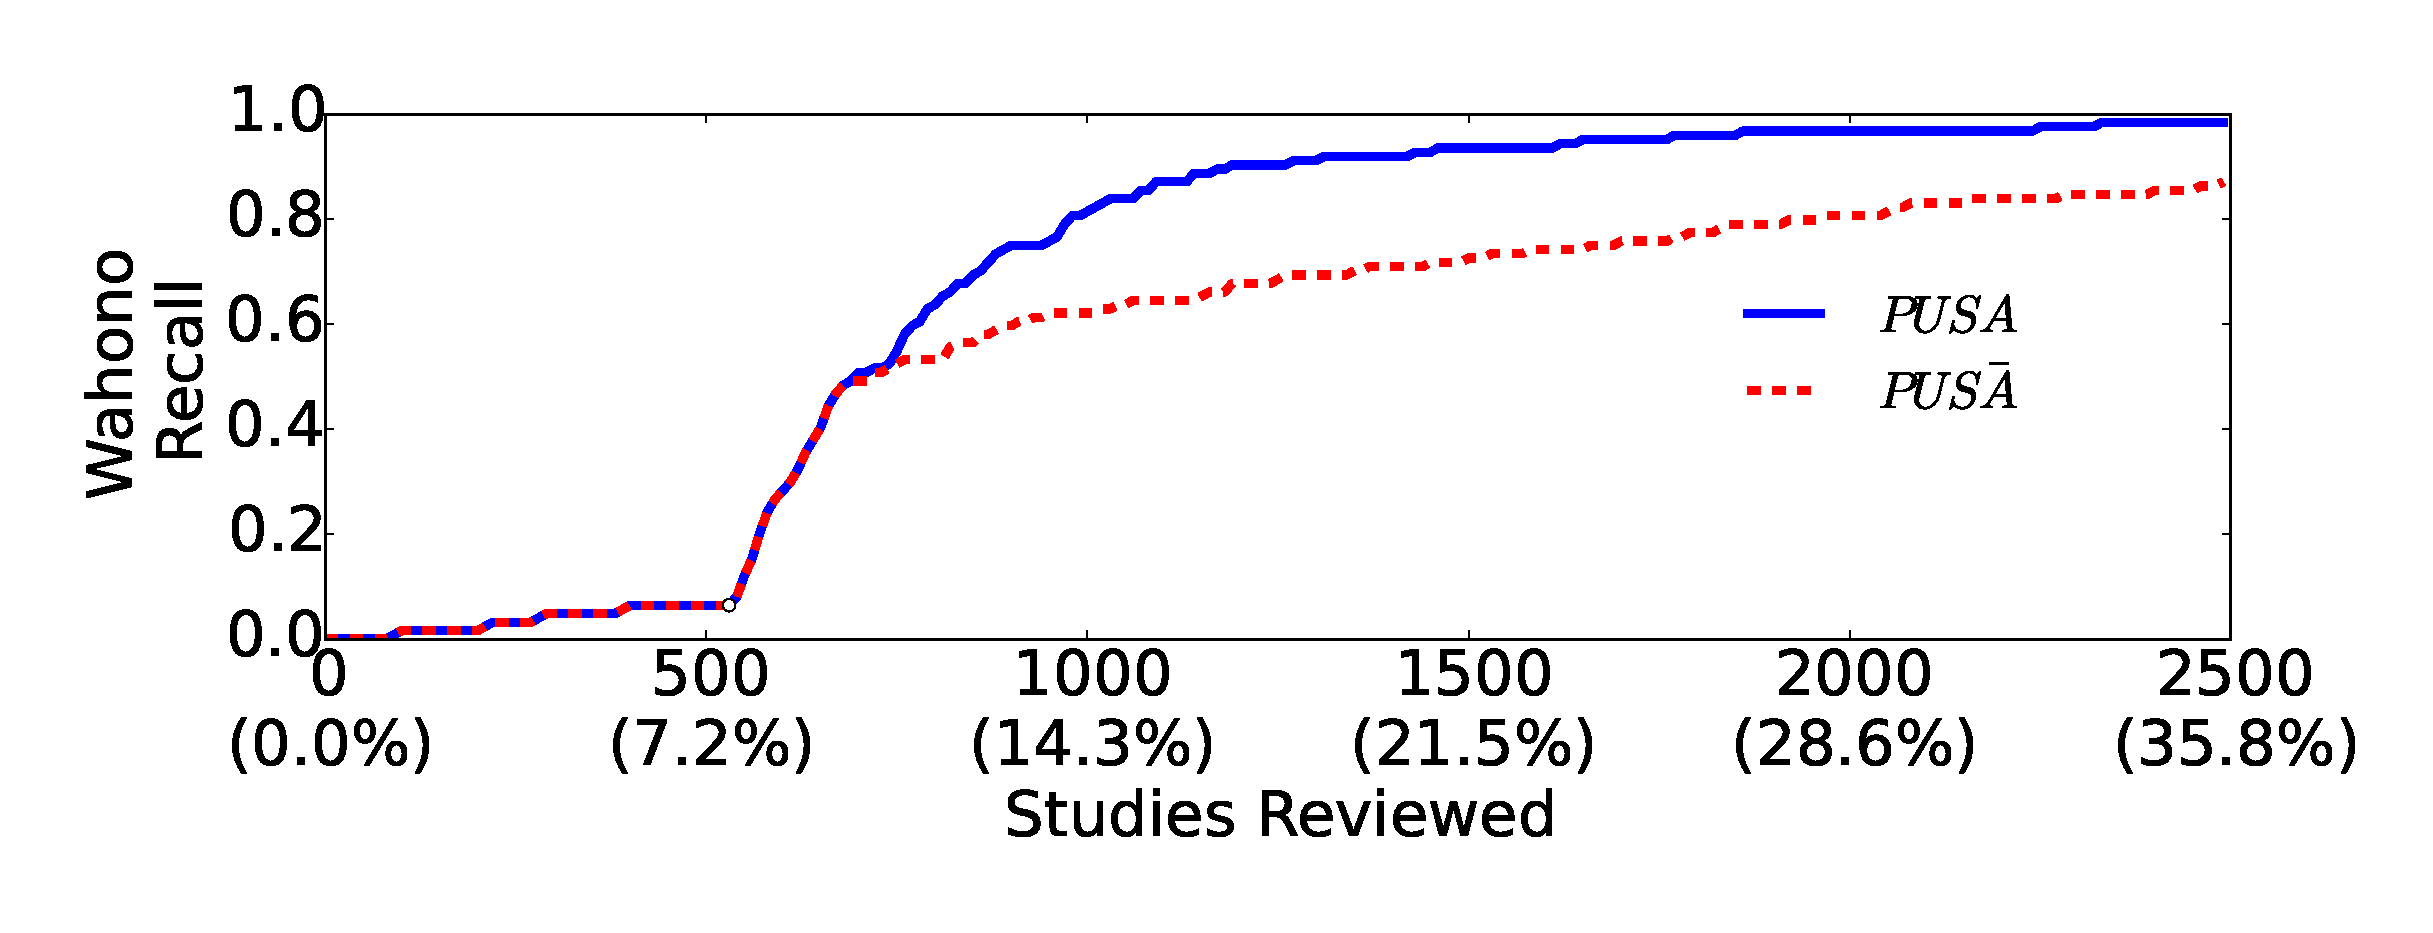
\includegraphics[width=0.48\linewidth]{IST_4_Wahono.eps}
        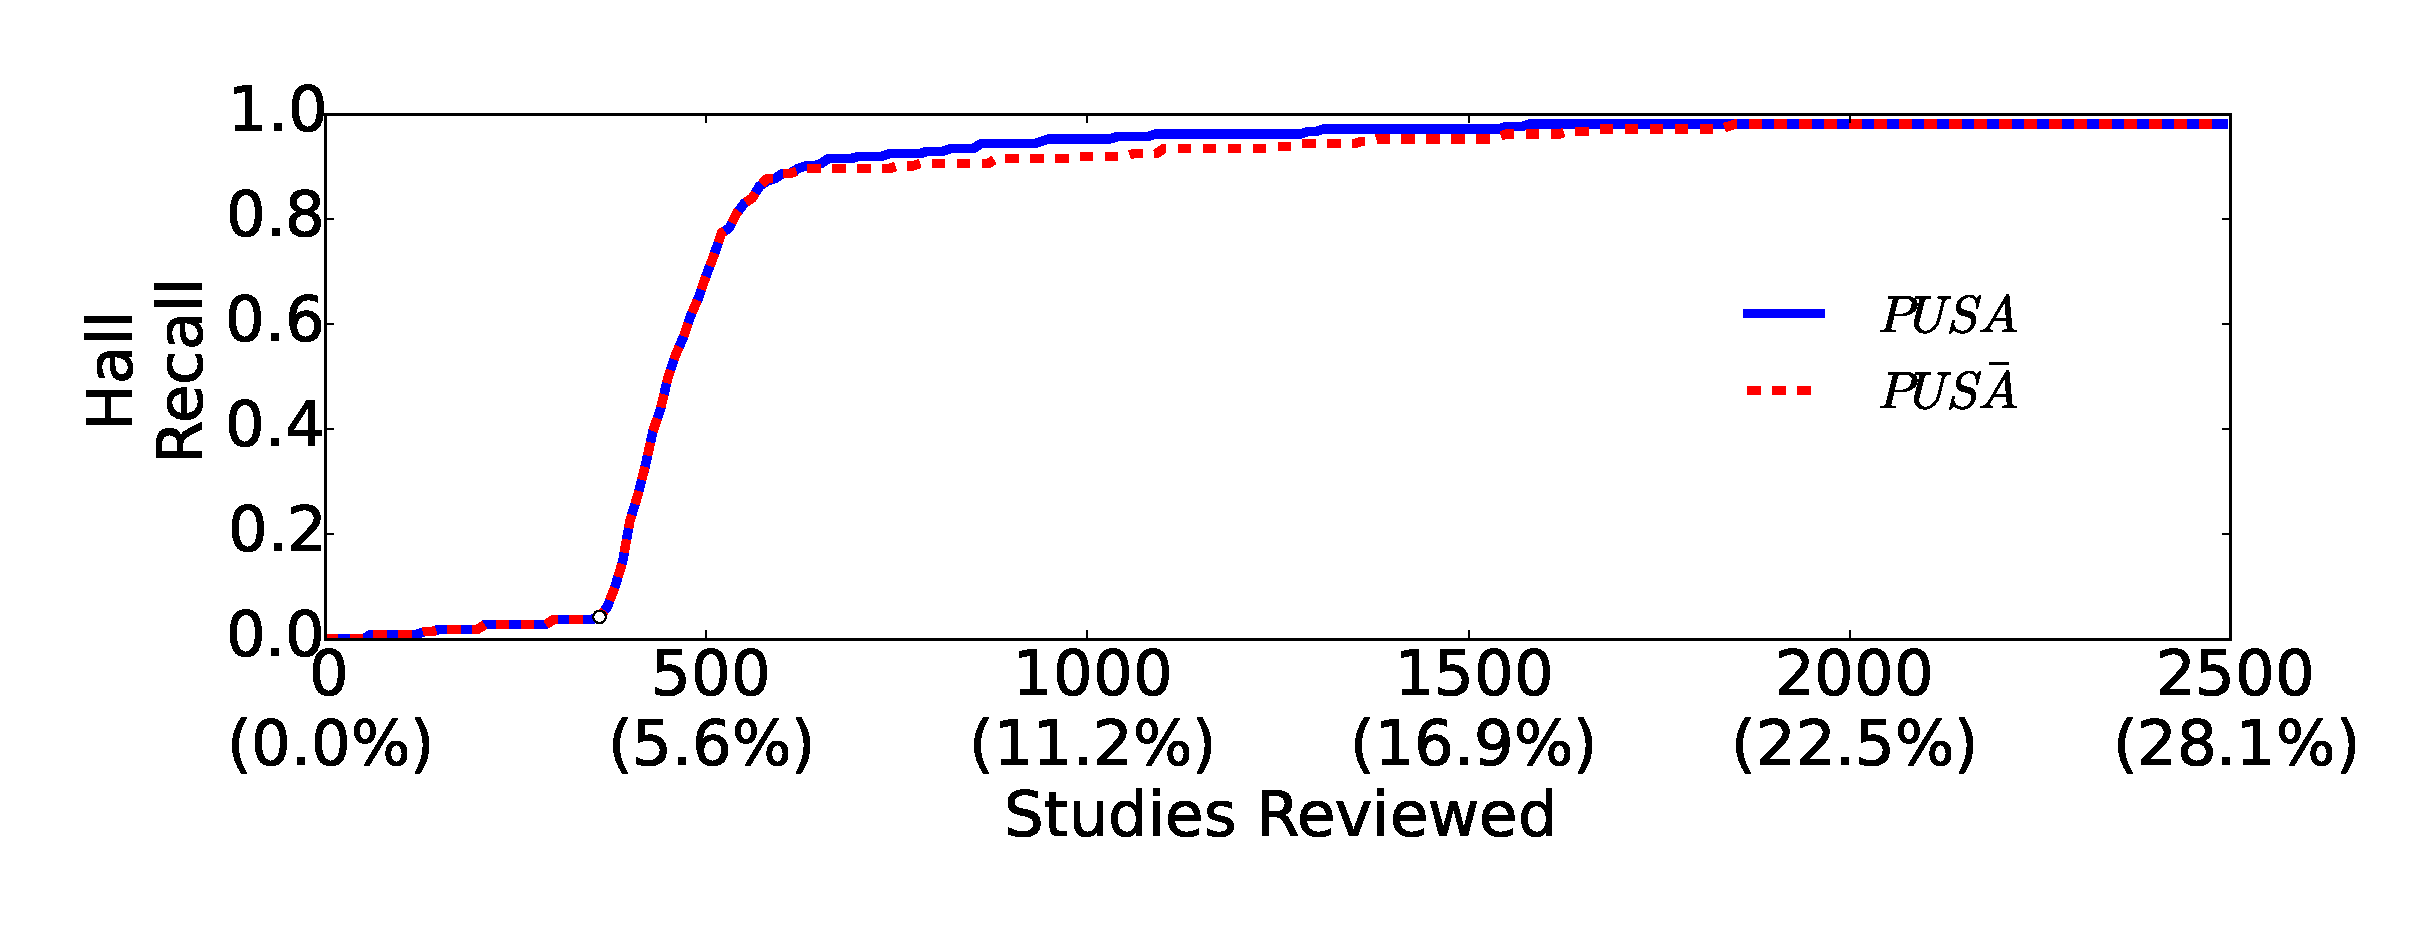
\includegraphics[width=0.48\linewidth]{IST_4_Hall.eps}
        \label{fig:4th}
    }
    \quad
    \subfigure[Is continuous learning useful? Comparison for \textbf{Code S}.]
    {
        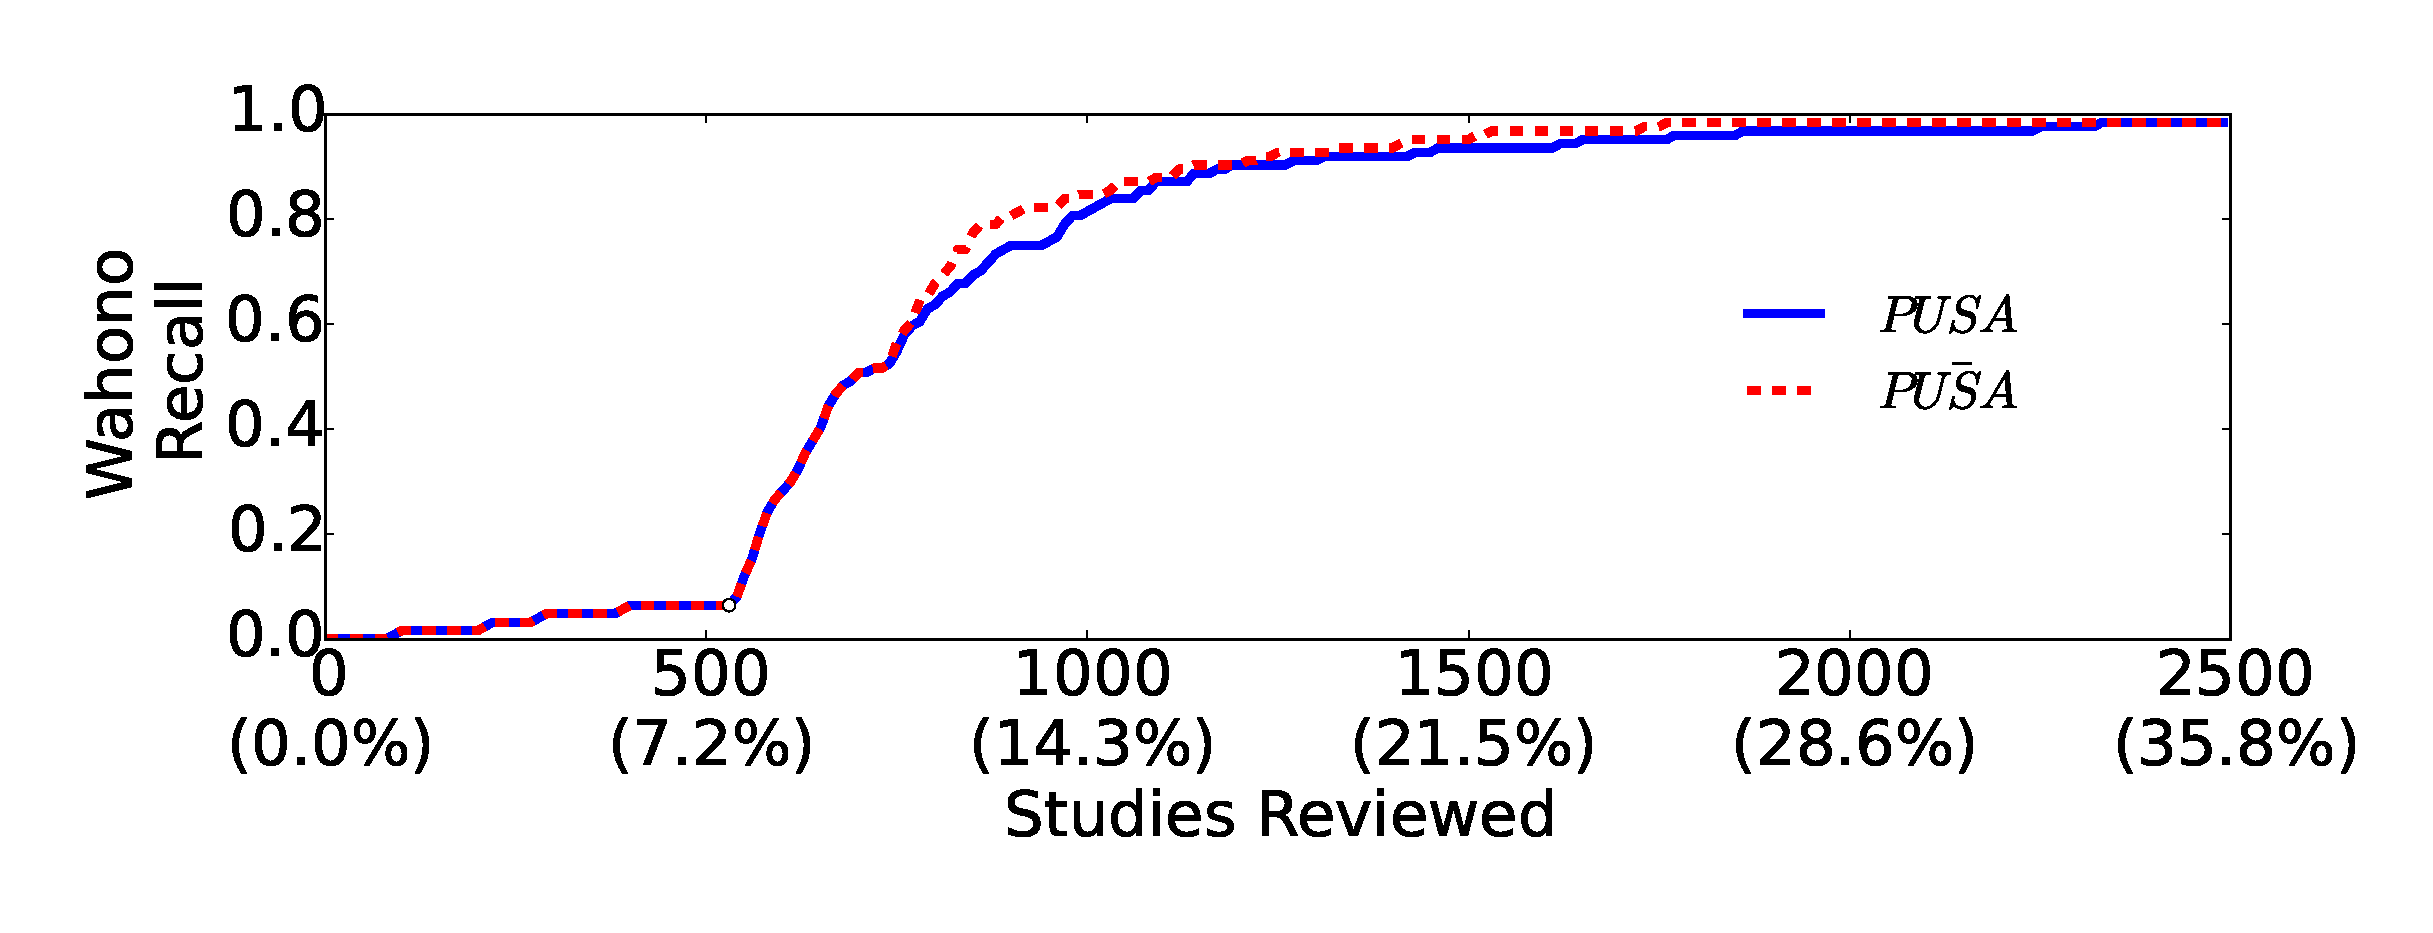
\includegraphics[width=0.48\linewidth]{IST_3_Wahono.eps}
        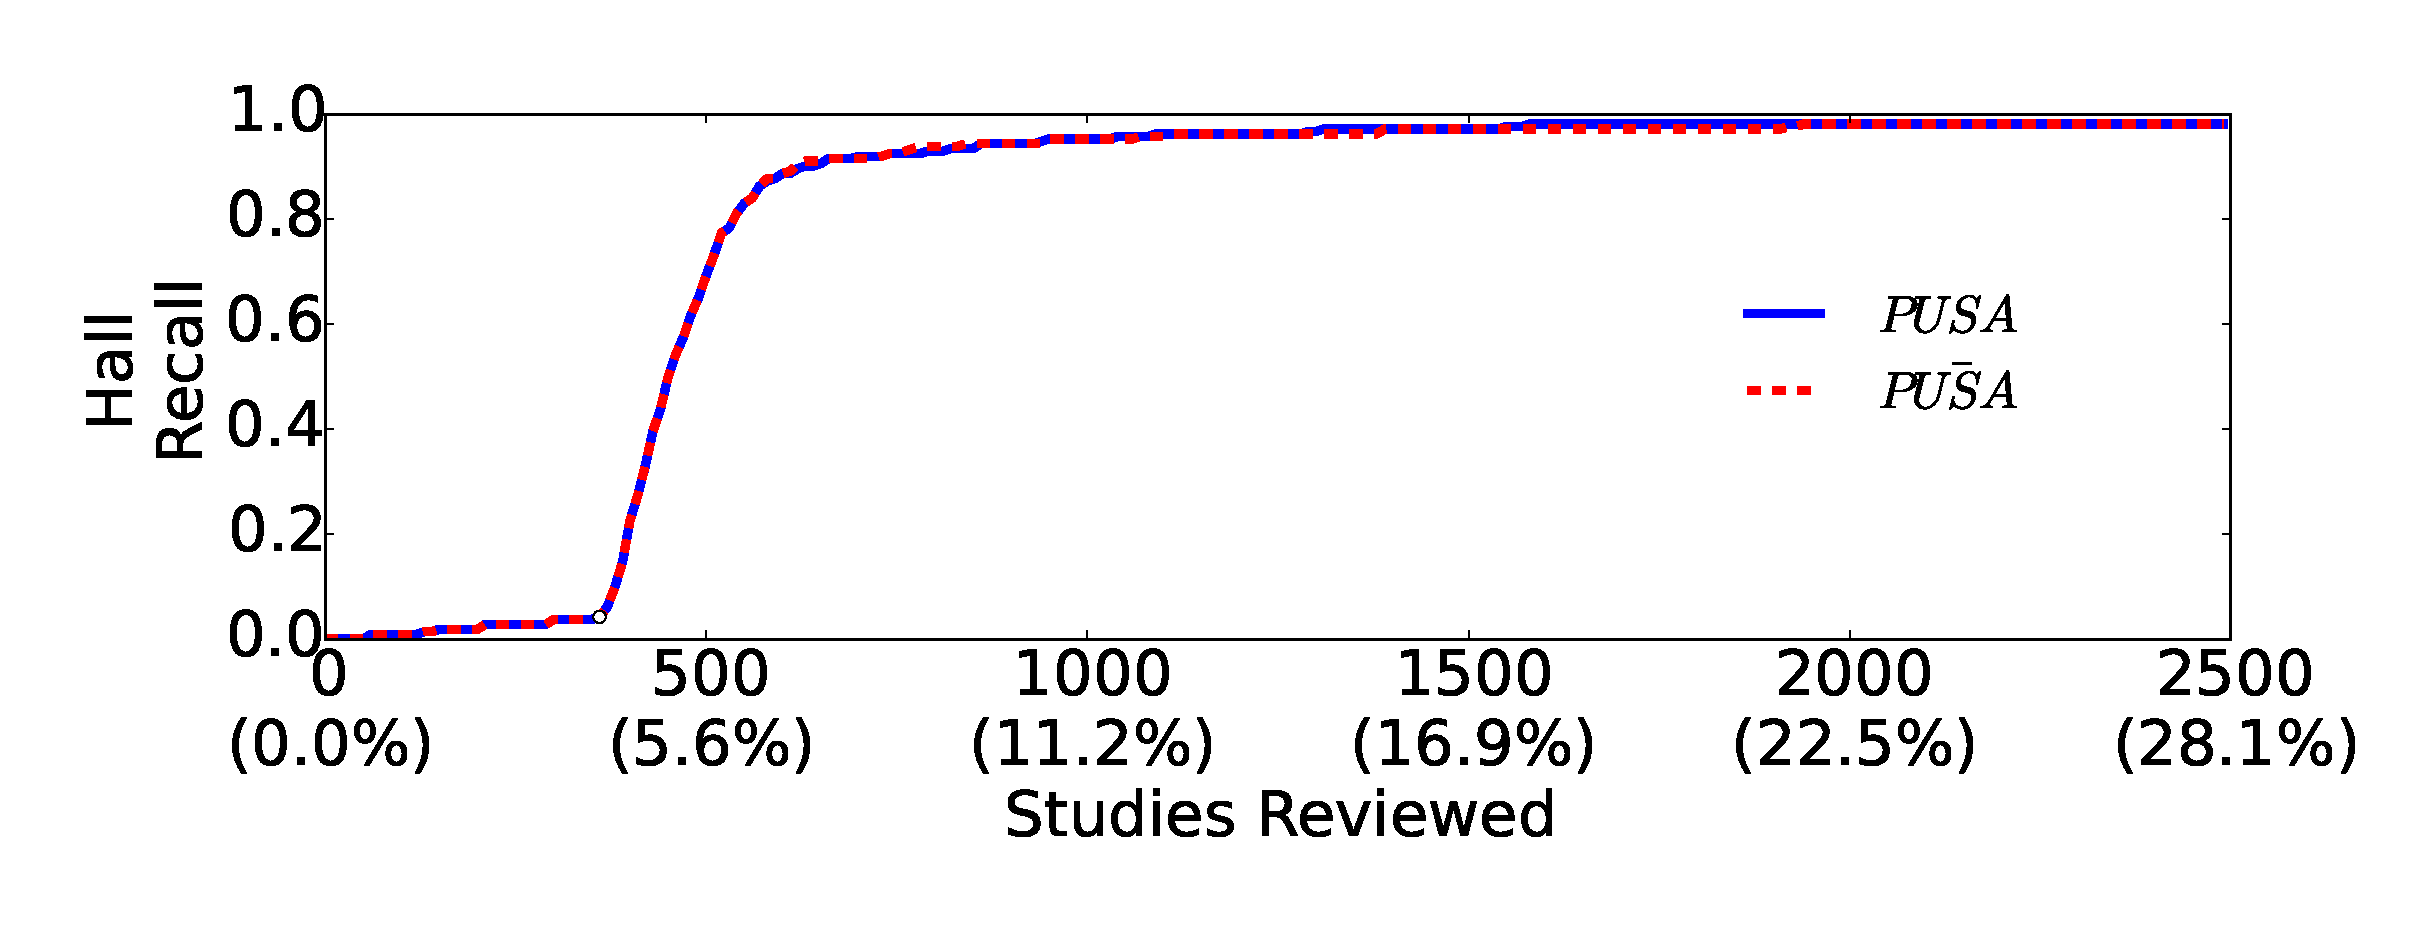
\includegraphics[width=0.48\linewidth]{IST_3_Hall.eps}
        \label{fig:3rd}
    }
    \quad
    \subfigure[Is uncertainty sampling useful? Comparison for \textbf{Code U}.]
    {
        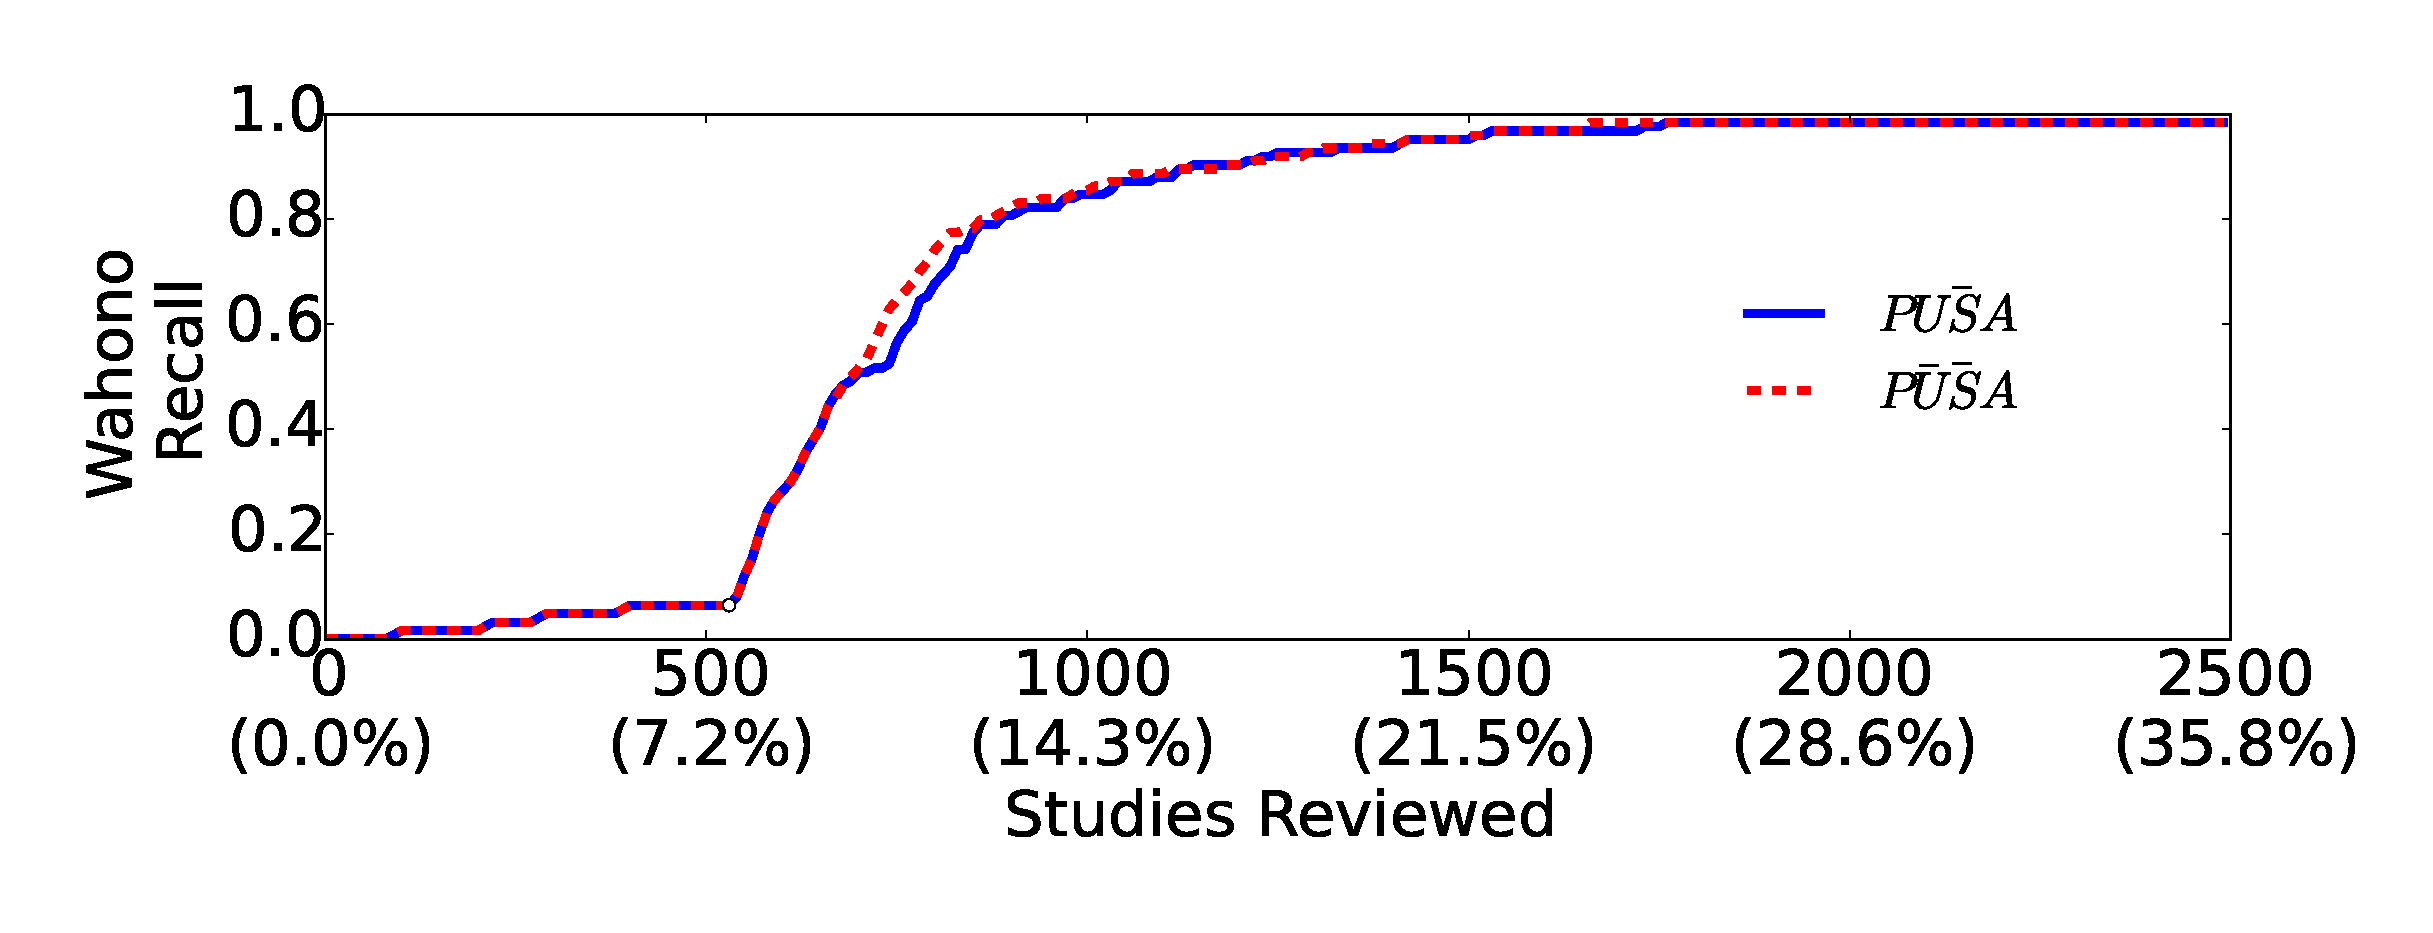
\includegraphics[width=0.48\linewidth]{IST_2_Wahono.eps}
        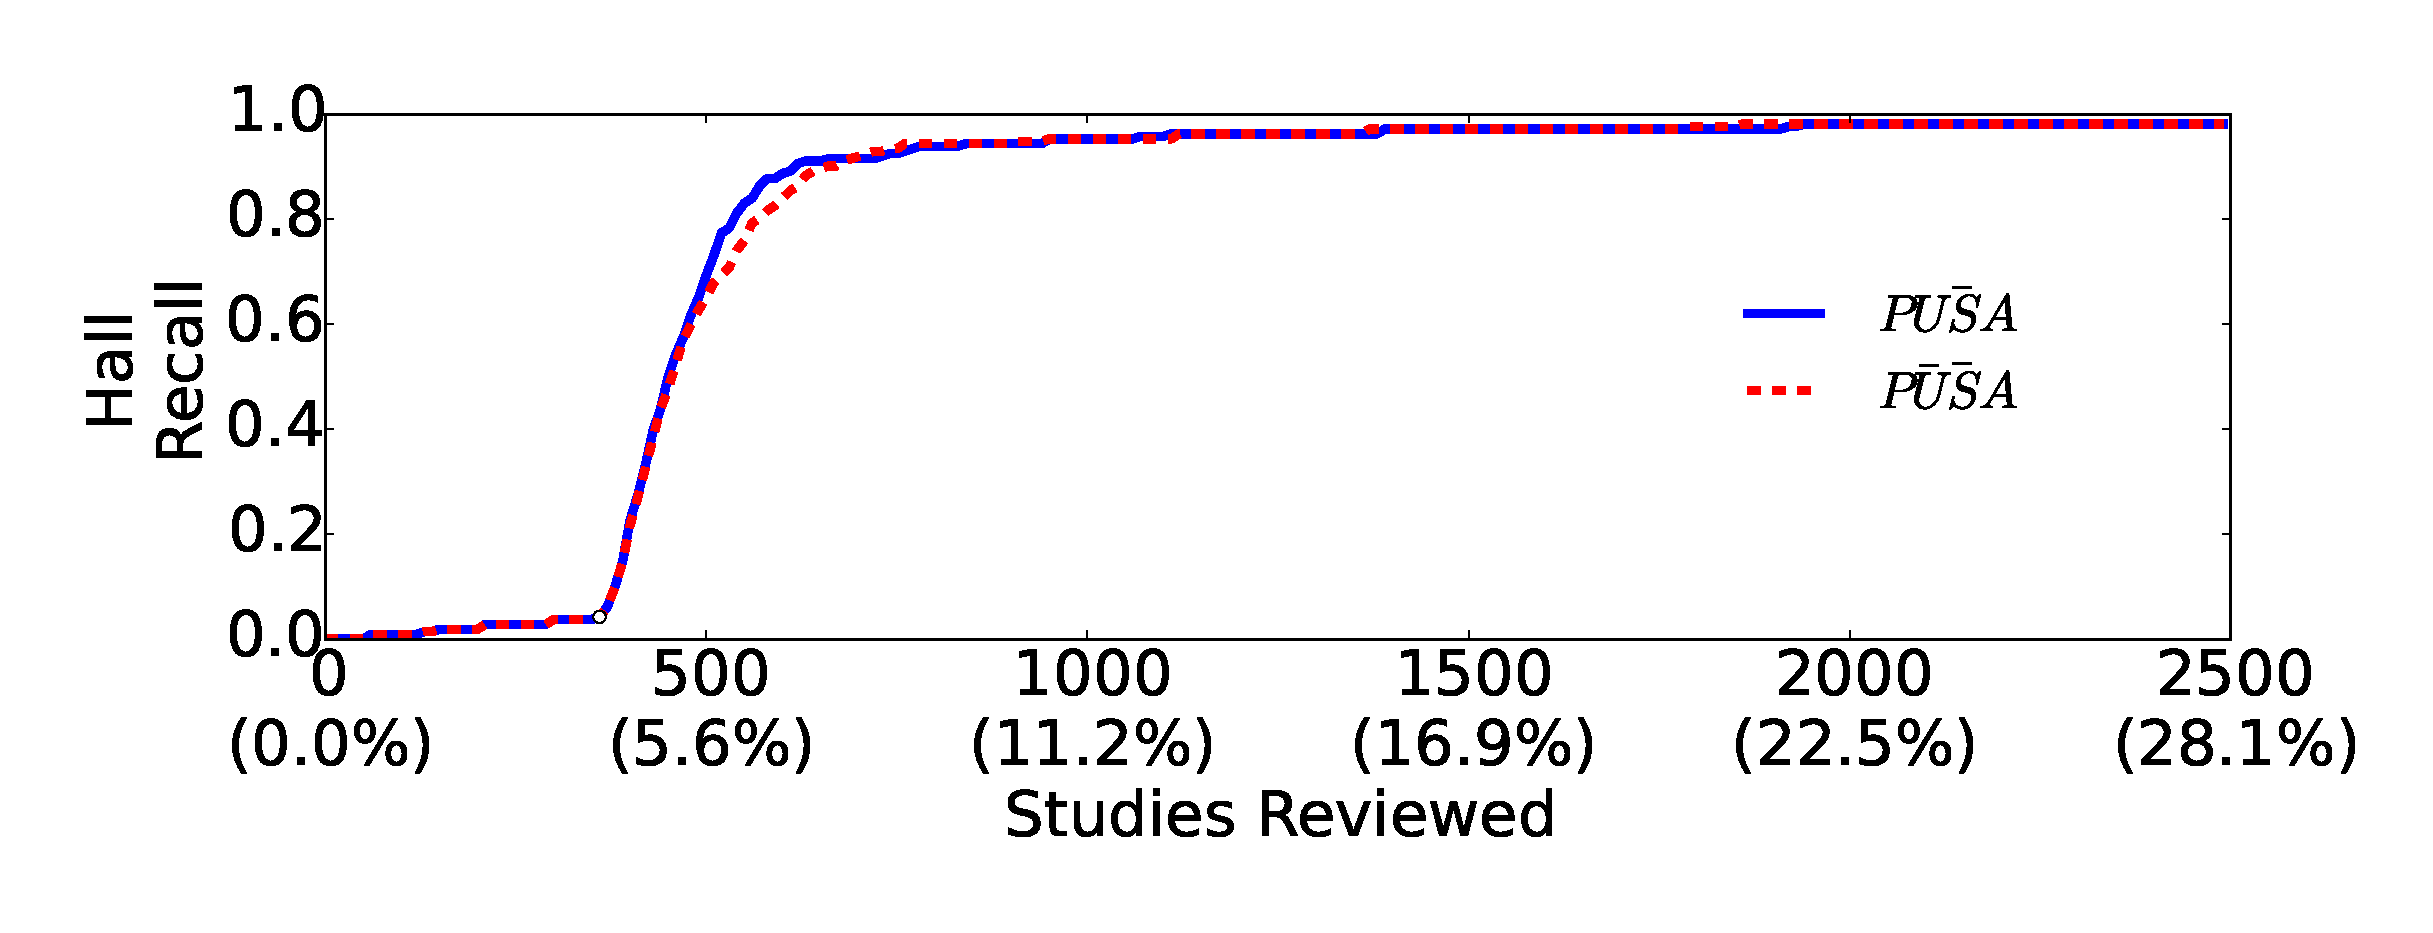
\includegraphics[width=0.48\linewidth]{IST_2_Hall.eps}
        \label{fig:2nd}
    }
    \quad
    \subfigure[Is patient useful? Comparison for \textbf{Code P}.]
    {
        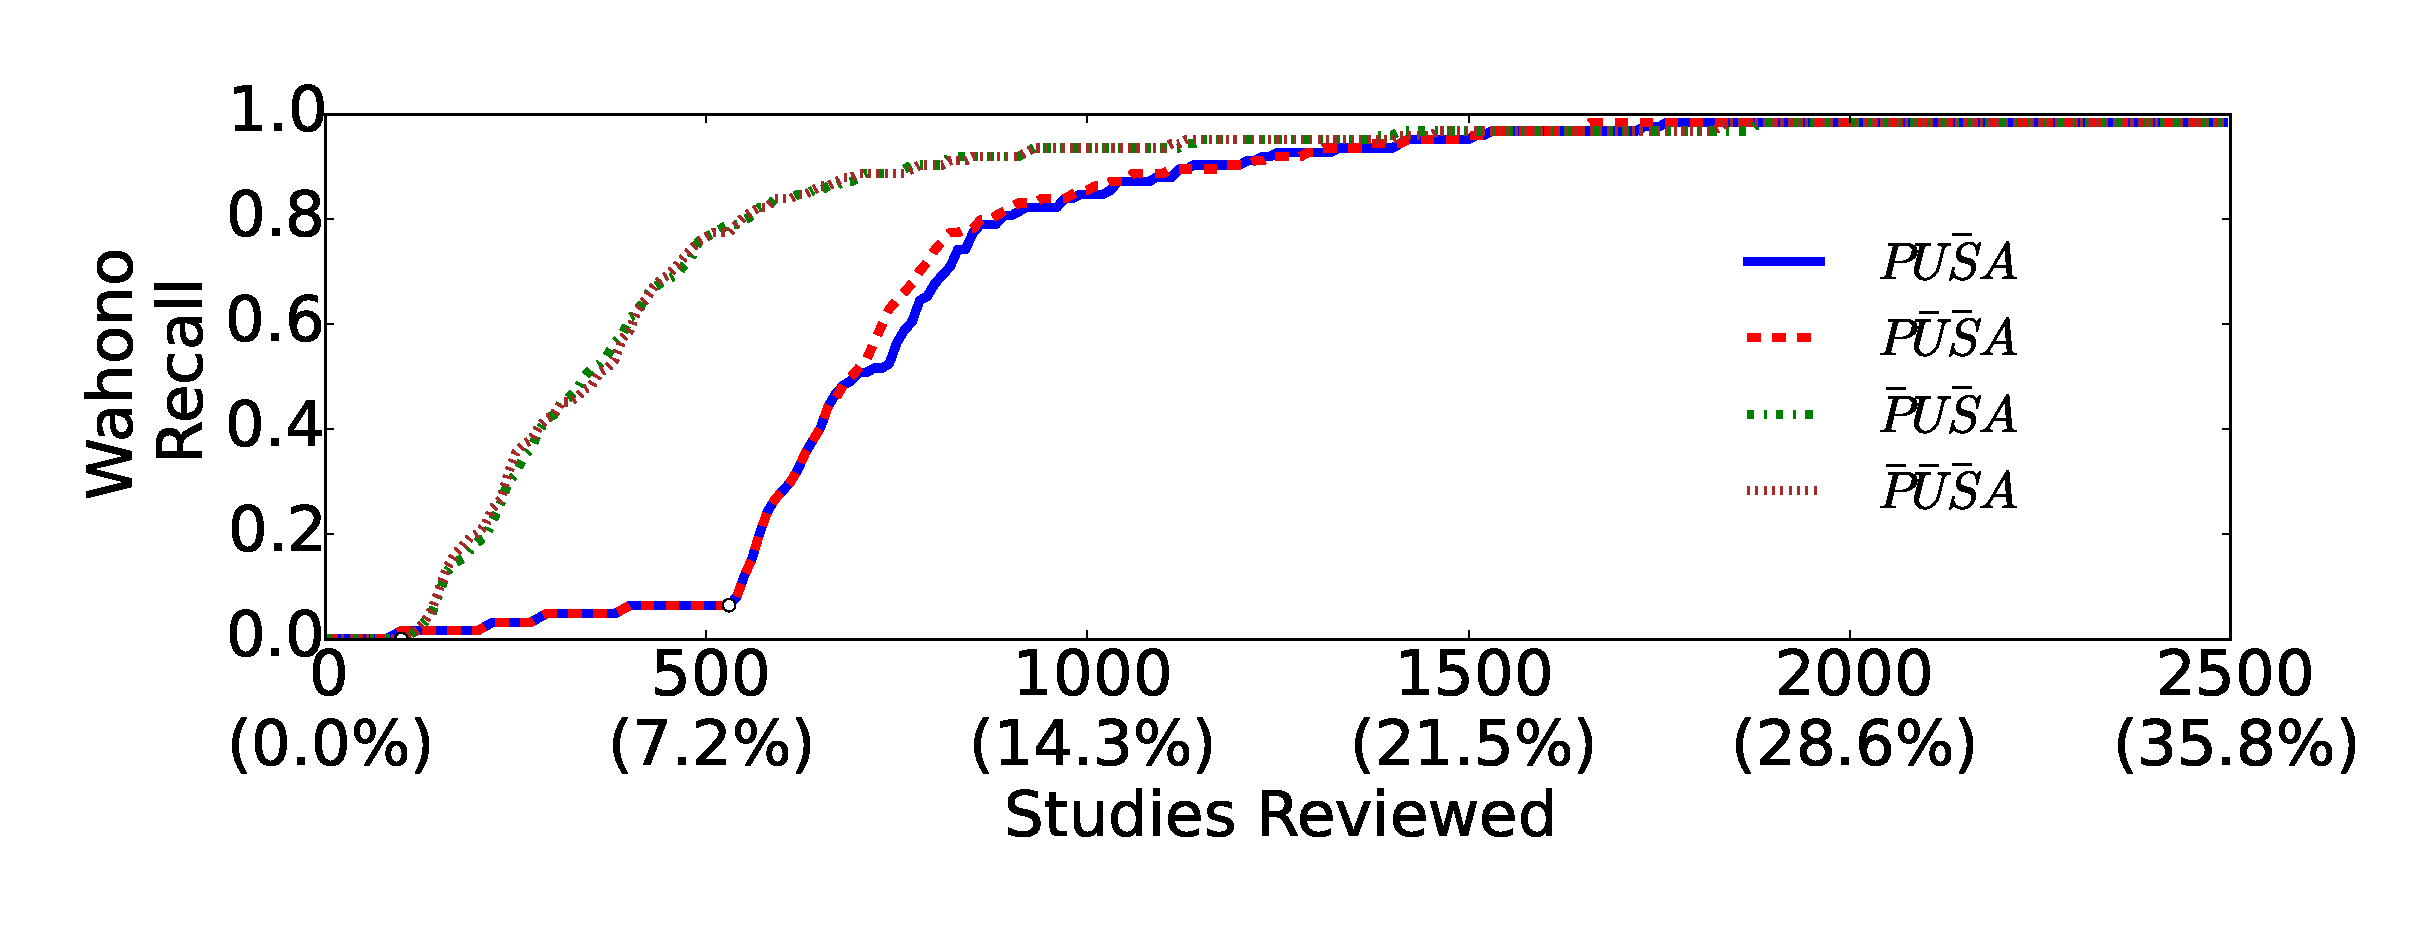
\includegraphics[width=0.48\linewidth]{IST_1_Wahono.eps}
        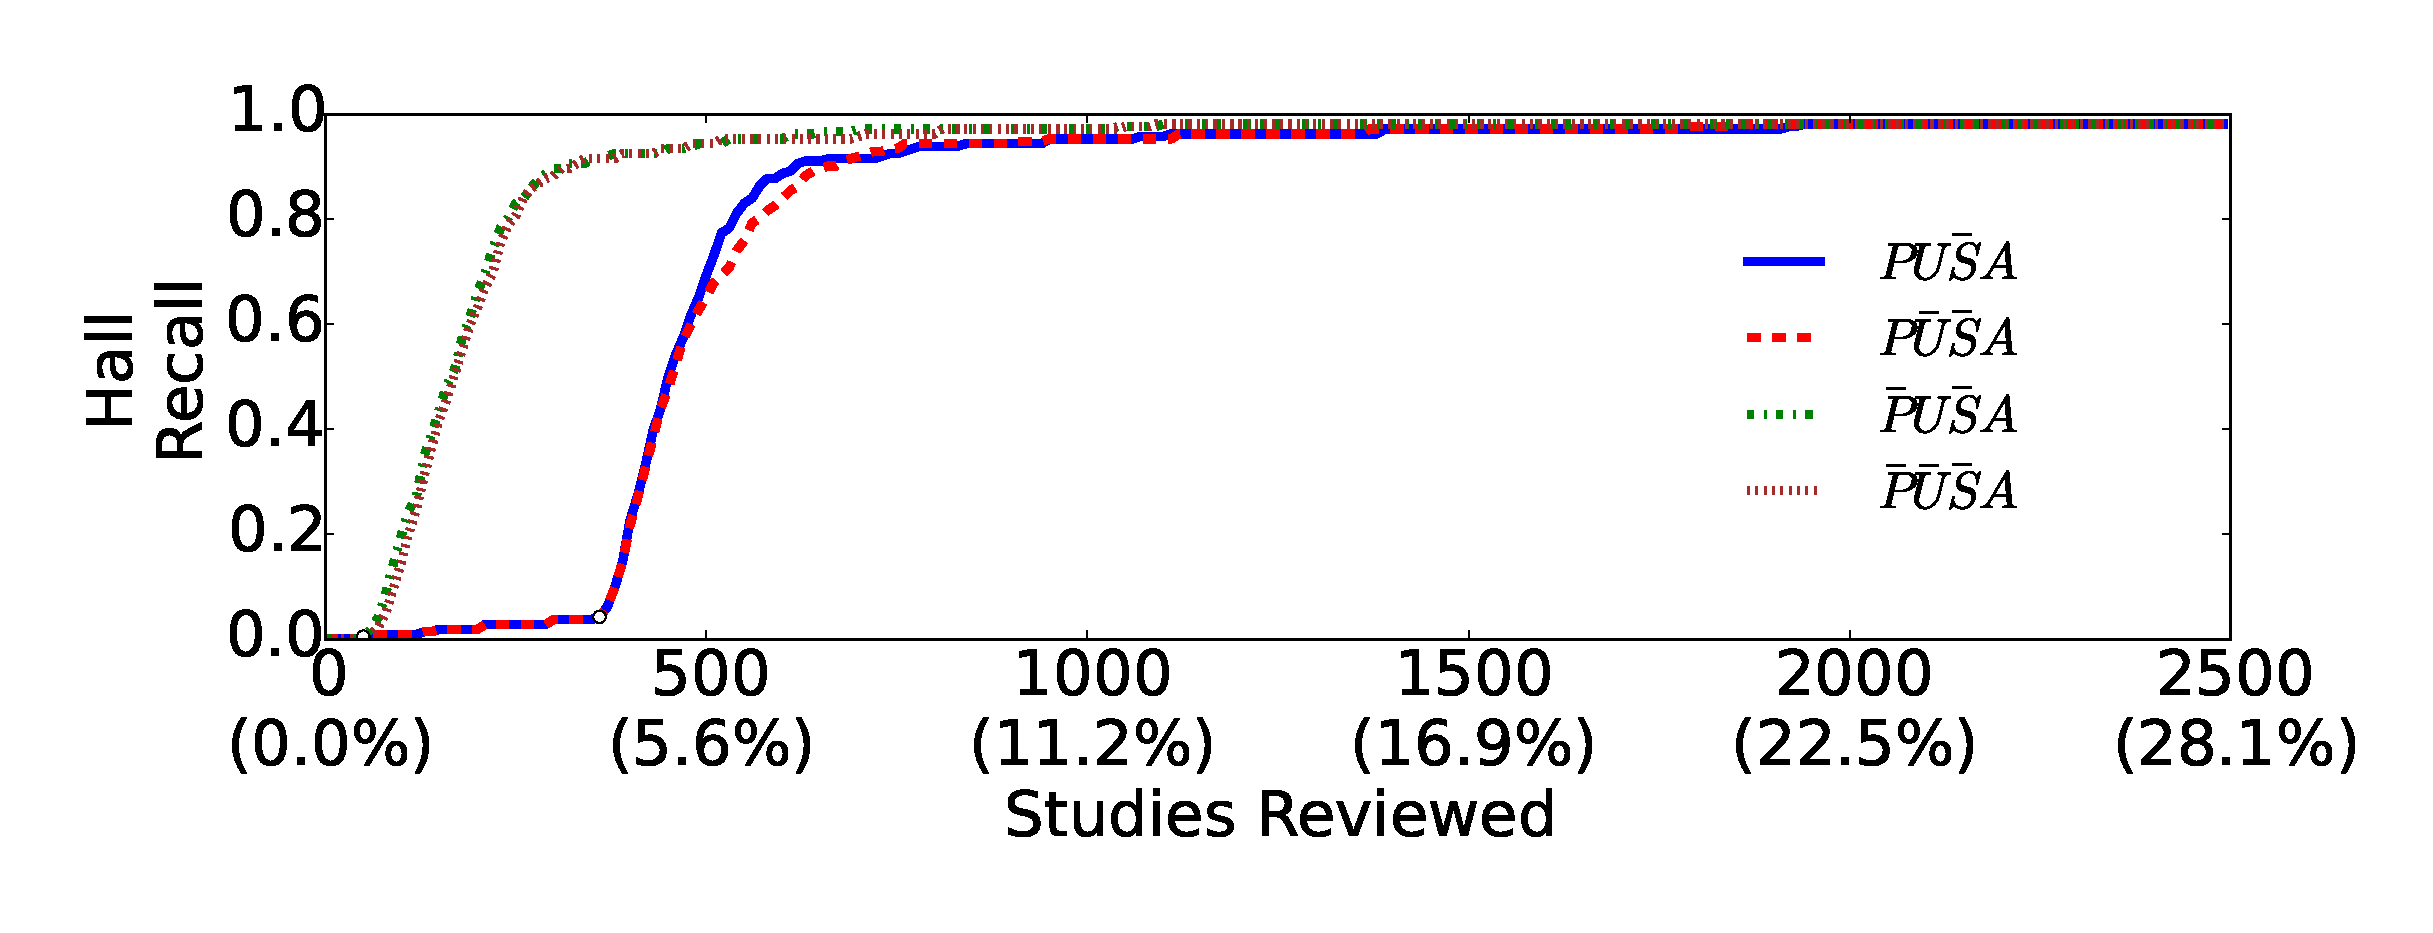
\includegraphics[width=0.48\linewidth]{IST_1_Hall.eps}
        \label{fig:1st}
    }
    
    
    \caption{(a) compares our recommended method FASTREAD with the two state-of-the-art methods, thereby answers RQ3. (b) to (e) are paired comparisons of different methods with results from Wahono data set on the left hand side and results from Hall data set on the right hand side. Each paired comparison answers one sub research question. (b) to (e) answer RQ3.1 to RQ3.4, respectively. Recall on Y axis represents the percentile of ``relevant'' studies being retrieved. X axis shows the number of studies reviewed with both absolute value and percentage of whole population in the brackets. Median values of recall in $30$ runs are presented. 
    }
    \label{fig:detail}
\end{figure*}

\begin{figure*}[ht]
    \centering
    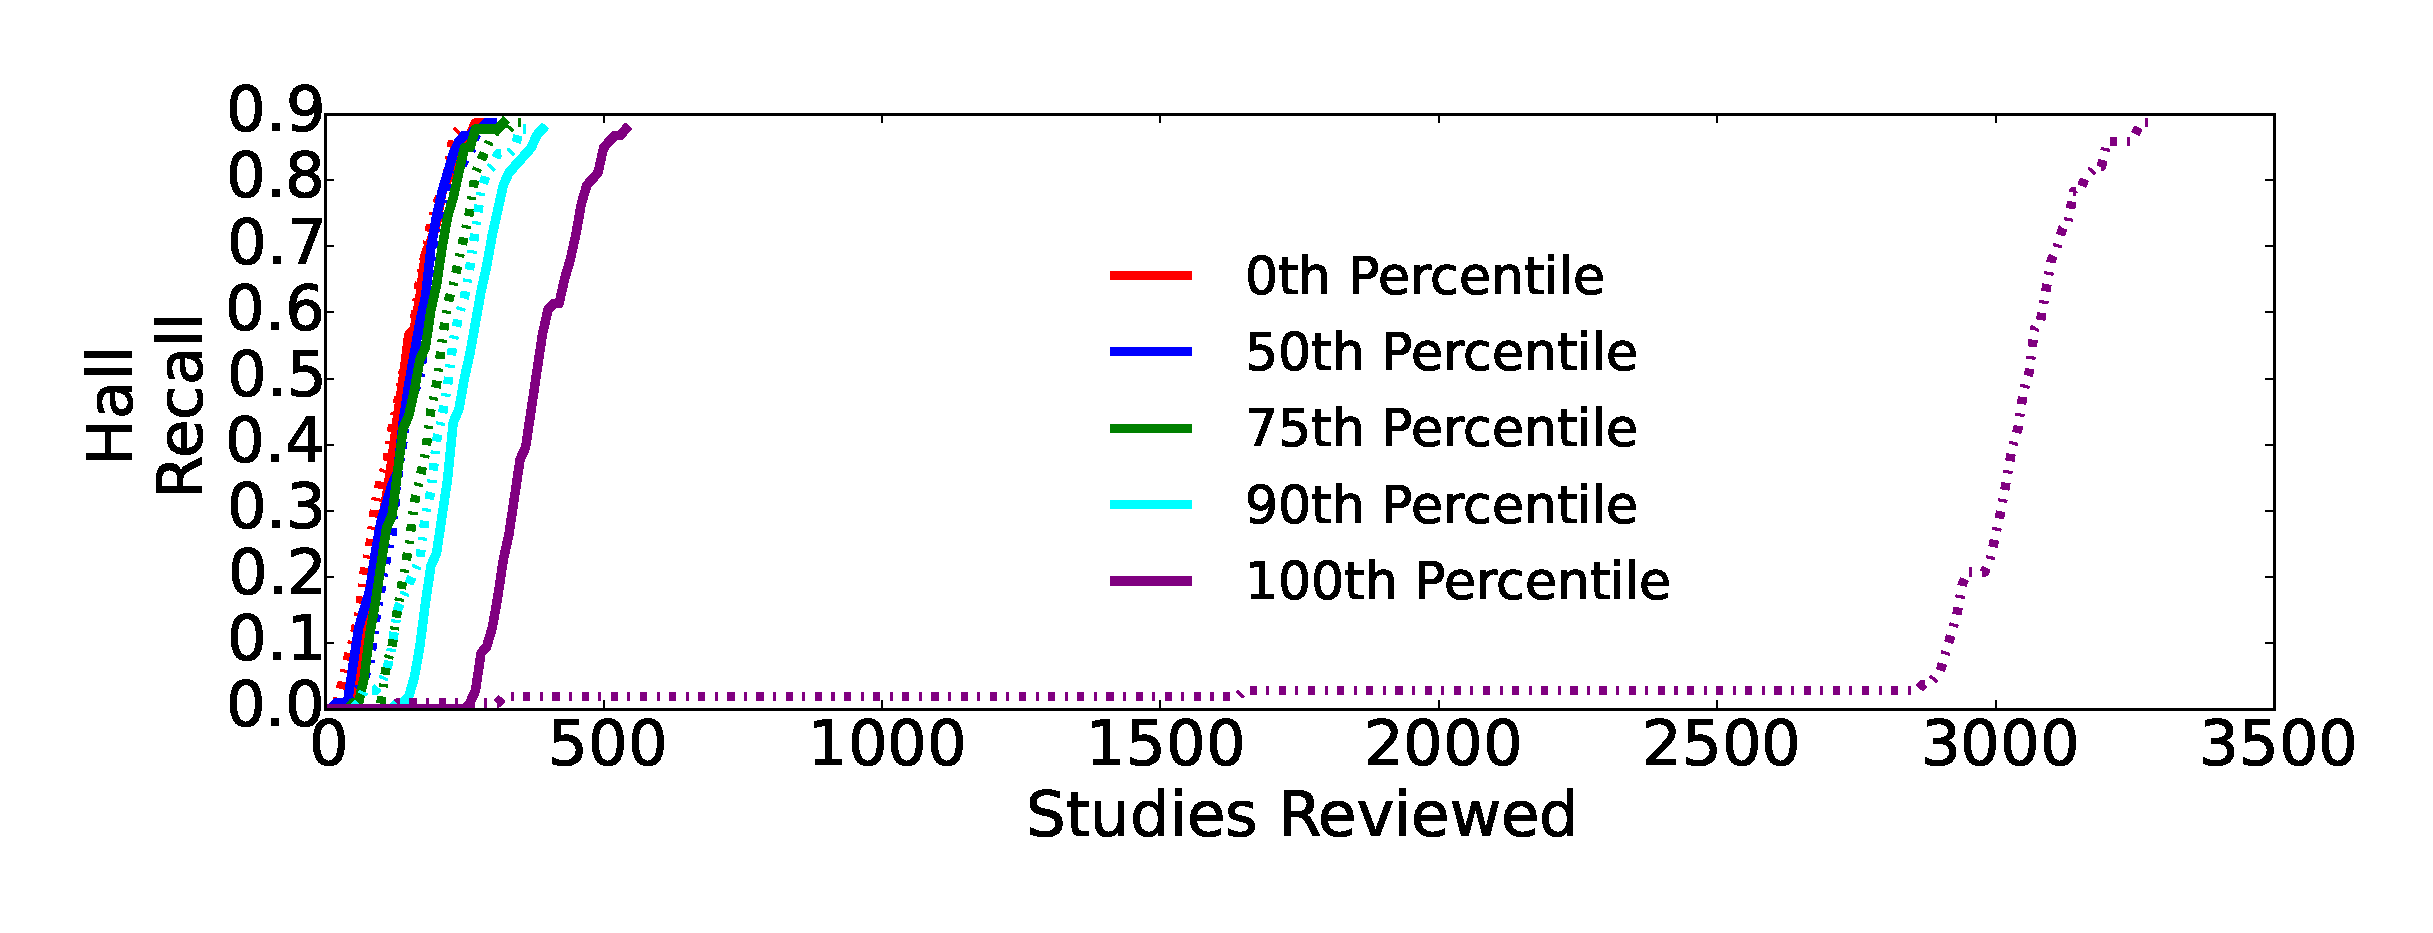
\includegraphics[width=0.48\linewidth]{percentile_Hall.eps}
    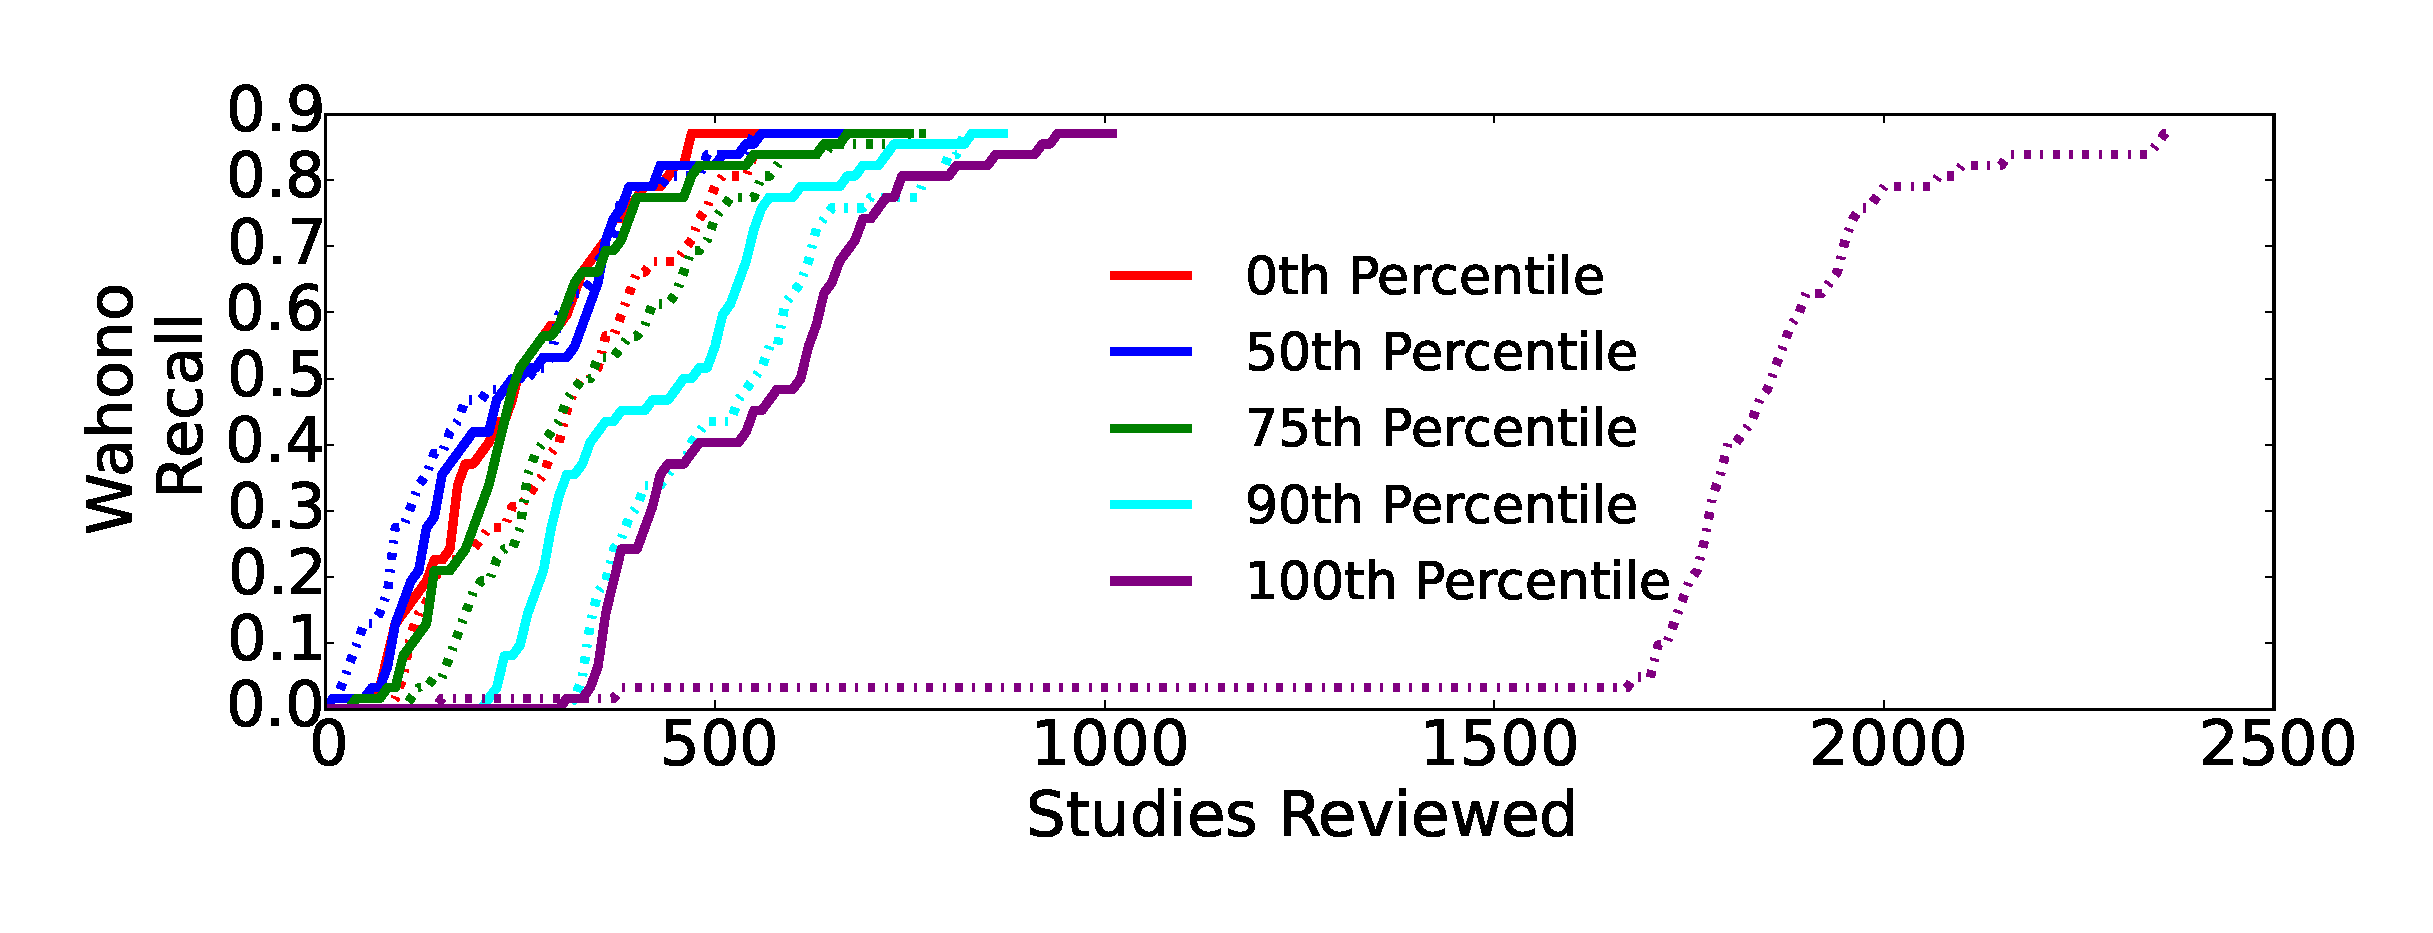
\includegraphics[width=0.48\linewidth]{percentile_Wahono.eps}
    \caption{Percentile graph of two treatments, $\bar{P}\bar{U}\bar{S}A$ as in solid lines and $\bar{P}U\bar{S}A$ as in dashed lines. All runs stop at $90\%$ recall for a fair comparison on review effort. RQ3.5 is answered here by comparing FASTREAD ($\bar{P}\bar{U}\bar{S}A$), the recommended treatment, with $\bar{P}U\bar{S}A$. The two treatments are similar regarding to median performance. However, according to the percentile graph, FASTREAD is better than $\bar{P}U\bar{S}A$ in terms of variance. Specifically, the worst case performance of FASTREAD is much better than that of $\bar{P}U\bar{S}A$.}
    \label{fig:percentile}
\end{figure*}




{\bf RQ3: Should we just adopt the state-of-the-art methods from other fields? Is it possible to build a better one by mixing and matching from those?}



By mixing and matching from the state-of-the-art methods, twelve different machine assisted reading methods are compared in our experiments, including patient active learning ($PUSA$) and continuous active learning ($\bar{P}\bar{U}\bar{S}\bar{A}$). Overall, $\bar{P}\bar{U}\bar{S}A$, which we call FASTREAD, outperforms other methods on both Wahono and Hall data set. Figure \ref{fig: baseline} shows the performance of FASTREAD comparing to the state-of-the-art methods. Additionally, a set of paired comparisons are made to further compare each component of the methods as shown in Figure~\ref{fig:4th}-\ref{fig:1st}.


\textbf{RQ3.1}: Is there a treatment better than the state-of-the-art treatments?

In order to answer RQ3.1, we compare the results of following three treatments:

\begin{itemize}
\item the recommended treatment of $\bar{P}\bar{U}\bar{S}A$ (FASTREAD),
\item the state-of-the-art evidence-based medicine treatment of $PUSA$ (patient active learning),
\item and the state-of-the-art e-discovery treatment of $\bar{P}\bar{U}\bar{S}\bar{A}$ (continuous active learning). 

Note that if FASTREAD performs the best then this would make us say ``yes'' to ``Is there a treatment better than the state-of-the-art treatments?''.
\end{itemize}

As demonstrated in Figure~\ref{fig: baseline}, FASTREAD outperforms others. Therefore the answer to RQ3.1 is yes, FASTREAD is better than the state-of-the-art treatments. 

Why FASTREAD? The following sub-research questions explain how we select the best treatment.

\textbf{RQ3.2}: Is aggressive undersampling useful?

Aggressive undersampling was first proposed along with patient active learning method in \cite{wallace2010semi}. Therefore we compare the results of two treatments:
\begin{itemize}
\item the ``no'' treatment of $PUS\bar{A}$ (without aggressive undersampling)
\item and the ``yes'' treatment of $PUSA$ (patient active learning). 

Note that if ``yes''
performs better then this would make us say ``yes'' to ``Is aggressive undersampling useful?''.
\end{itemize}
As shown in Figure~\ref{fig:4th}, ``yes'' outperforms ``no'' on on both data sets. Therefore the answer to RQ3.2 is yes, aggressive undersampling is useful and plays an important role in machine assisted reading.

\textbf{RQ3.3}: Is continuous learning useful?

The winner from last paired comparison, $PUSA$ (patient active learning) suggests that learning should be stopped after classifier is ``stable''. On the other hand, continuous active learning in \cite{cormack2014evaluation} suggests that we should never stop learning. Therefore we compare the results of two treatments:

\begin{itemize}
\item the ``no'' treatment of $PUSA$ (patient active learning, stops learning after ``stable''.)
\item and the ``yes'' treatment of $PU\bar{S}A$ (continue learning). 

Note that if ``yes''
performs better then this would make us say ``yes'' to ``Is continuous learning useful?''.
\end{itemize}

According to Figure~\ref{fig:3rd}, ``yes'' performs a little bit better than ``no'' on Wahono data set. Although there is no clear winner, we recommend continuous learning due to its ability to tackle concept drift and continuous update of SLR. Therefore the answer to RQ3.3 is that continuous learning has no significant impact on performance, but it is suggested because of other reasons.

\textbf{RQ3.4}: Is uncertainty sampling useful?

The winner from last paired comparison, $PU\bar{S}A$ suggests that uncertainty sampling should be applied in the early stage to build the classifier. On the other hand, continuous active learning suggests that uncertainty sampling is not necessary. Therefore we compare the results of two treatments:

\begin{itemize}
\item the ``no'' treatment of $PU\bar{S}A$ (with uncertainty sampling)
\item and the ``yes'' treatment of $P\bar{U}\bar{S}A$ (without uncertainty sampling). 

Note that if ``yes''
performs better then this would make us say ``yes'' to ``Is uncertainty sampling useful?''.
\end{itemize}

According to Figure~\ref{fig:2nd}, there are no clear differences in performance between these two treatments. Both are kept for the next round of paired comparison. The answer to RQ3.4 is that uncertainty sampling is not a must-have. This is a shocking result as most of the literature about active learning suggest that uncertainty sampling is indispensable in fast building up a good model. However, the objective of machine assisted reading is different from general active learning task. In stead of trying to build a classifier as good as possible, machine assisted reading seeks methods to retrieve almost every ``relevant'' studies with candidate studies reviewed as few as possible. This particular objective of machine assisted reading makes certainty sampling equally or even more competitive to uncertainty sampling. Similar results have been found in \cite{cormack2014evaluation}.

\textbf{RQ3.5}: Is patient useful?

The winners from last paired comparison, $PU\bar{S}A$ and $P\bar{U}\bar{S}A$ suggest that we should wait until enough ``relevant'' examples have been retrieved before training an SVM model. On the other hand, continuous active learning suggests that training should start as soon as
one ``relevant'' example retrieved. Therefore, we compare the results of four treatments:

\begin{itemize}
\item the ``no'' treatment of $\bar{P}U\bar{S}A$ (without patient),
\item the ``no'' treatment of $\bar{P}\bar{U}\bar{S}A$ (without patient),
\item the ``yes'' treatment of $P\bar{U}\bar{S}A$ (with patient), 
\item and the ``yes'' treatment of $PU\bar{S}A$ (with patient). 

Note that if both ``yes'' treatments performs better then this would make us say ``yes'' to ``Is patient useful?''.
\end{itemize}

According to Figure~\ref{fig:1st}, ``no'' treatments are clear winners. The two ``no'' treatments, $\bar{P}U\bar{S}A$ and $\bar{P}\bar{U}\bar{S}A$, have similar performance. Thus the answer to RQ3.5 is no, patient is not useful, training the SVM model as soon as ONE ``relevant'' example retrieved performs better. This result is also surprising. A reasonable explanation can still be drawn from the objective of machine assisted reading, as RQ3.5. By sacrificing some performance of early SVM model, we gain advantage of finding more ``relevant'' studies earlier. Similar results are also found in \cite{cormack2014evaluation}.

\textbf{RQ3.6}: What is the recommended treatment in terms of median performance?

Considering all the above comparisons, we end up with two winners among the twelve treatments in terms of median performance, $\bar{P}U\bar{S}A$ and $\bar{P}\bar{U}\bar{S}A$. These two treatments are indistinguishable in terms of median performance and both outperforms the state-of-the-art treatments.

\textbf{RQ3.7}: What is the recommended treatment in terms of variance?

The variances of both $\bar{P}U\bar{S}A$ and $\bar{P}\bar{U}\bar{S}A$ in $30$ runs are shown in Figure~\ref{fig:percentile}, in which the best and worst cases, along with 50, 75, 90 percentile cases are plotted. Although $\bar{P}U\bar{S}A$ and $\bar{P}\bar{U}\bar{S}A$ have similar median performance, the variance of $\bar{P}\bar{U}\bar{S}A$ is less than that of $\bar{P}U\bar{S}A$ as shown in Figure~\ref{fig:percentile}. Especially in the worst cases, $\bar{P}\bar{U}\bar{S}A$ performs significantly better than $\bar{P}U\bar{S}A$ (purple curves). Thus the answer to RQ3.7 is that the recommended treatment is $\bar{P}\bar{U}\bar{S}A$, which we call FASTREAD.

As shown as solid lines in Figure~\ref{fig:percentile}, variance of FASTREAD are extremely low in $75\%$ of the cases, where reviewers need to review $5\%$ (/$10\%$) to retrieve $90\%$ of the ``relevant'' studies in Hall (/Wahono) data set. Causing by the instability of random sampling, in $10\%$ of the cases, the review cost is increased by $50\%$, while in the worst case result, the review effort is doubled. The reason behind is that the number of studies reviewed before the first ``relevant'' one appears can vary. For example, the prevalence of ``relevant'' studies in Hall is $106/8911=0.012$, there is a $(1-0.12)^{200}=9\%$ of chance that the first $200$ studies reviewed has no ``relevant'' studies in it. How to reduce variance when building the seed set is a problem and we are planning to address it in our future work.

To sum up: the recommended machine assisted reading treatment for machine assisted primary study selection is FASTREAD ($\bar{P}\bar{U}\bar{S}A$), which randomly samples until {\em ONE}
``relevant'' study has been retrieved, then keeps certainty sampling until $M=30$ ``relevant'' studies are retrieved, after that keeps certainty sampling with aggressive undersampling. It is among the best performance treatments, and it outperforms both the state-of-art treatments in evidence-based medicine and e-discovery. Continuous learning also empower it the capability to handle concept drift and continuous update of SLR. 

\begin{lesson}
    No, we should not just adopt the state-of-the-art methods from other fields. Yes, we build a better method called FASTREAD by mixing and matching from the state-of-the-art methods.
\end{lesson}

\begin{figure}[th]
    \centering
    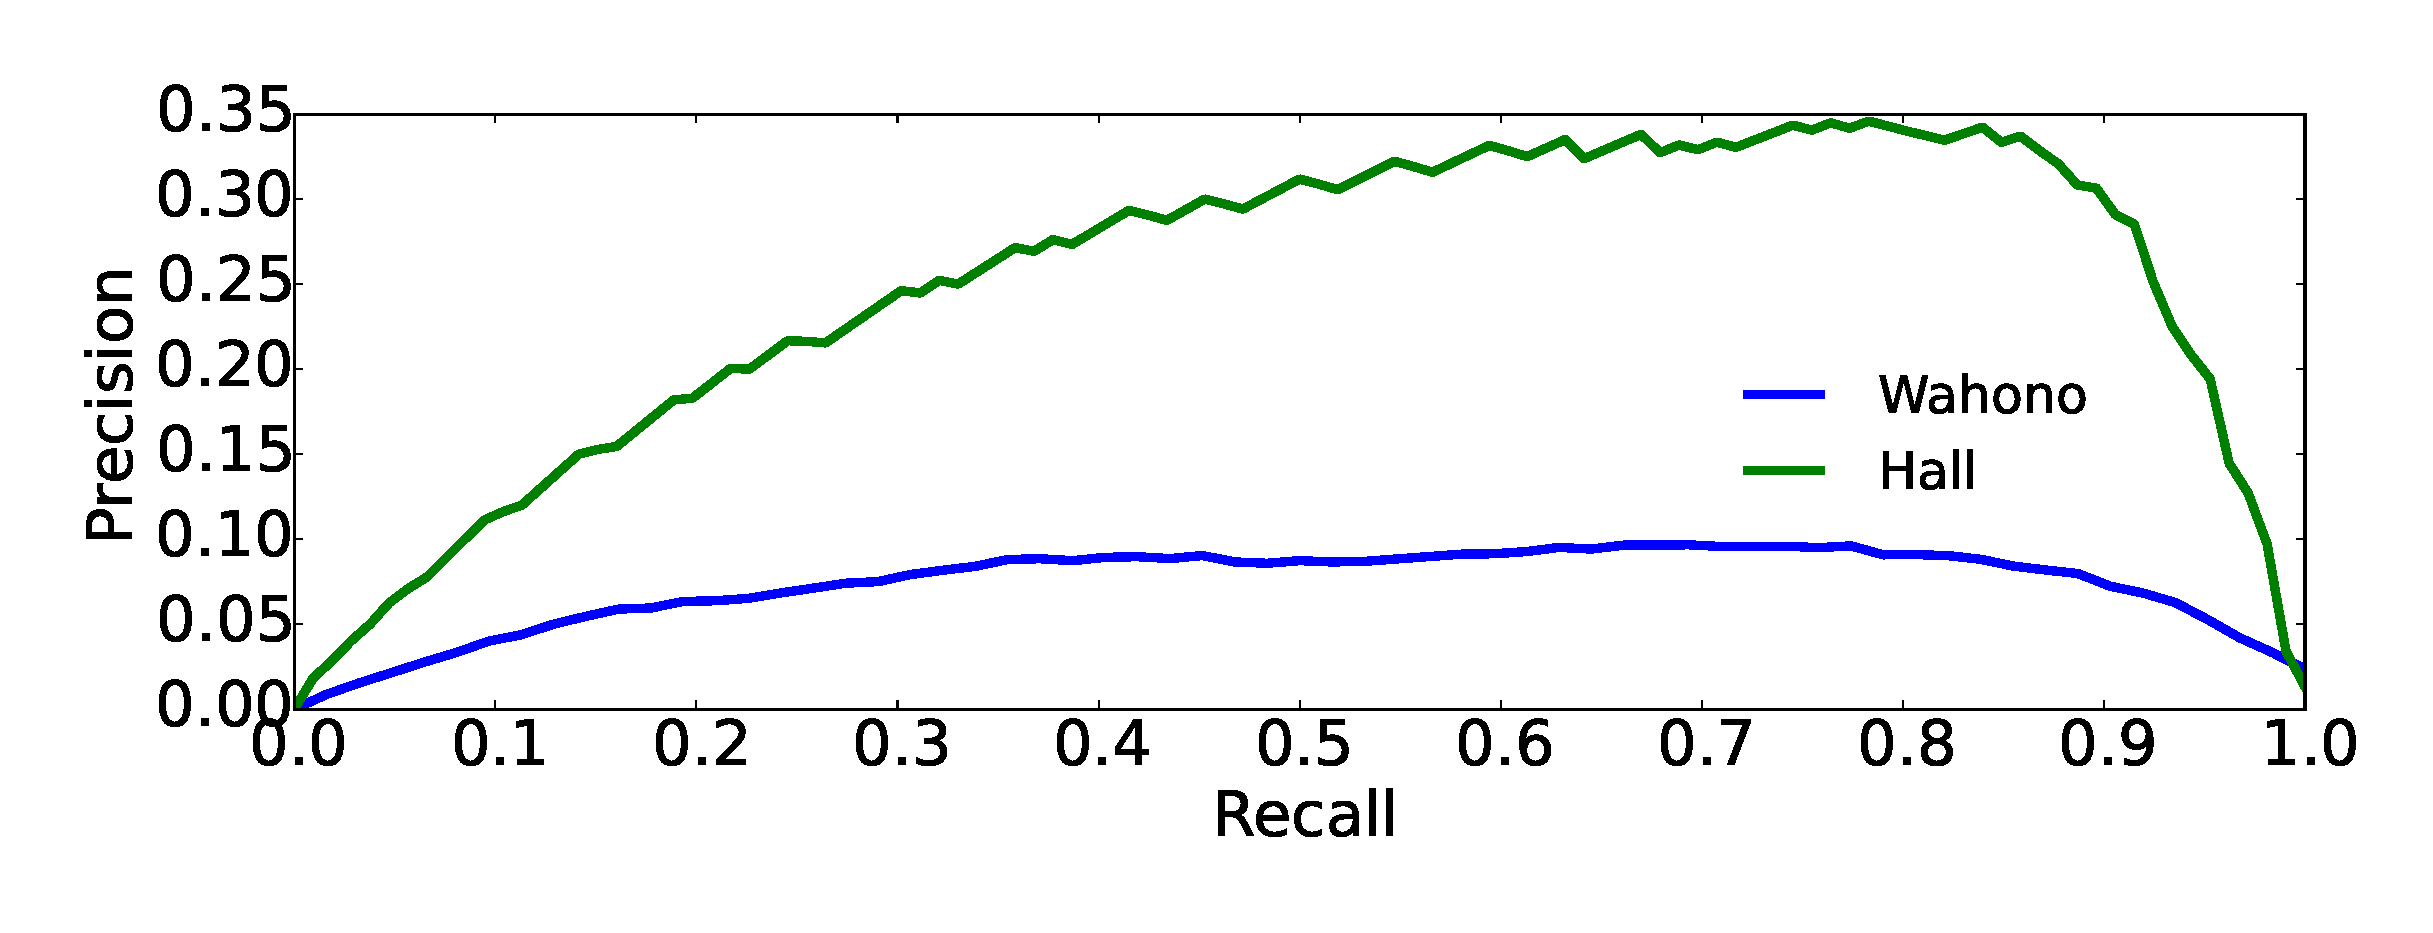
\includegraphics[width=\linewidth]{PoR.eps}
    \caption{The precision of FASTREAD for different target recall. Highest precisions are achieved around 0.8 recall. After 0.9 recall, precisions drop dramatically.}
    \label{fig:precision}
\end{figure}



\textbf{RQ4: How much effort can FASTREAD save in an SLR?}

In order to answer RQ4, let's first answer the following research questions:

\textbf{RQ4.1}: When should FASTREAD stop?

$100\%$ recall can never be achieved unless all the candidate studies have been reviewed, thus sacrificing recall (completeness) is a must if we want to save review effort in SLR. Precision, (number of ``relevant'' studies retrieved) / (number of studies reviewed), measures the efficiency of the review. The higher the precision, the more efficient the review is. Therefore precision should be taken into consideration since our goal is higher recall on less review effort. According to Figure~\ref{fig:precision}, highest precision can be achieved on both sets if FASTREAD stops at around $80\%$ recall. After $90\%$ recall, precision drops dramatically. Typically, increasing recall from $90\%$ to $95\%$ will double the review cost of FASTREAD. As a result, we suggest FASTREAD to stop at $90\%$ recall where precision just starts to drop. In practice, recall is unavailable. Thus another practical reason for stopping at $90\%$ recall is that, with the precision drop, reviewer can sense the plateau and know when to stop. 

\textbf{RQ4.2}: How many studies need to be reviewed at $90\%$ recall?

On Hall data set, in order to achieve a $90\%$ recall, a median value of $310$ studies need to be reviewed, which is $3.5\%$ of the total population.

On Wahono data set, in order to achieve a $90\%$ recall, a median value of $680$ studies need to be reviewed, which is $9.7\%$ of the total population.


\begin{figure}[th]
    \centering
    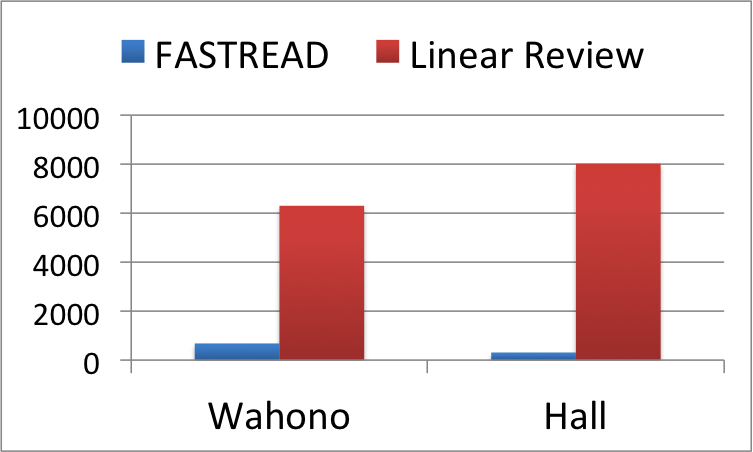
\includegraphics[width=.7\linewidth]{Reviewcost.png}    
    \caption{Number of studies reviewed to achieve $90\%$ recall.}
    \label{fig:reviewcost}
\end{figure}

To sum up, for RQ4, only hundreds of studies (around $5$ to $10\%$ of the total population) need to be reviewed in order to retrieve $90\%$ of the ``relevant'' studies, which implies a $90\%$ of review effort saved by FASTREAD. Figure~\ref{fig:reviewcost} compares the review cost for $90\%$ recall of FASTREAD and linear review.

\begin{lesson}
    Our results suggest that FASTREAD can save $90\%$ of the review effort while retrieving $90\%$ of the ``relevant'' studies.
\end{lesson}

\begin{figure*}[!t]
    \centering
    \subfigure[Input format]
    {
        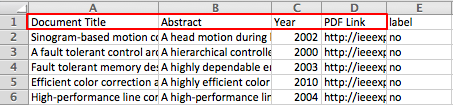
\includegraphics[width=0.48\linewidth]{Input.png}\label{fig:input}
    }
    \subfigure[Output format]
    {
        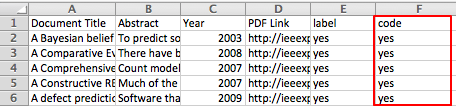
\includegraphics[width=0.48\linewidth]{Output.png}\label{fig:output}
    }    
    
    \caption{Data format for MAR tool.}
    \label{fig:csv}
\end{figure*}
\begin{figure*}[!t]
    \centering
    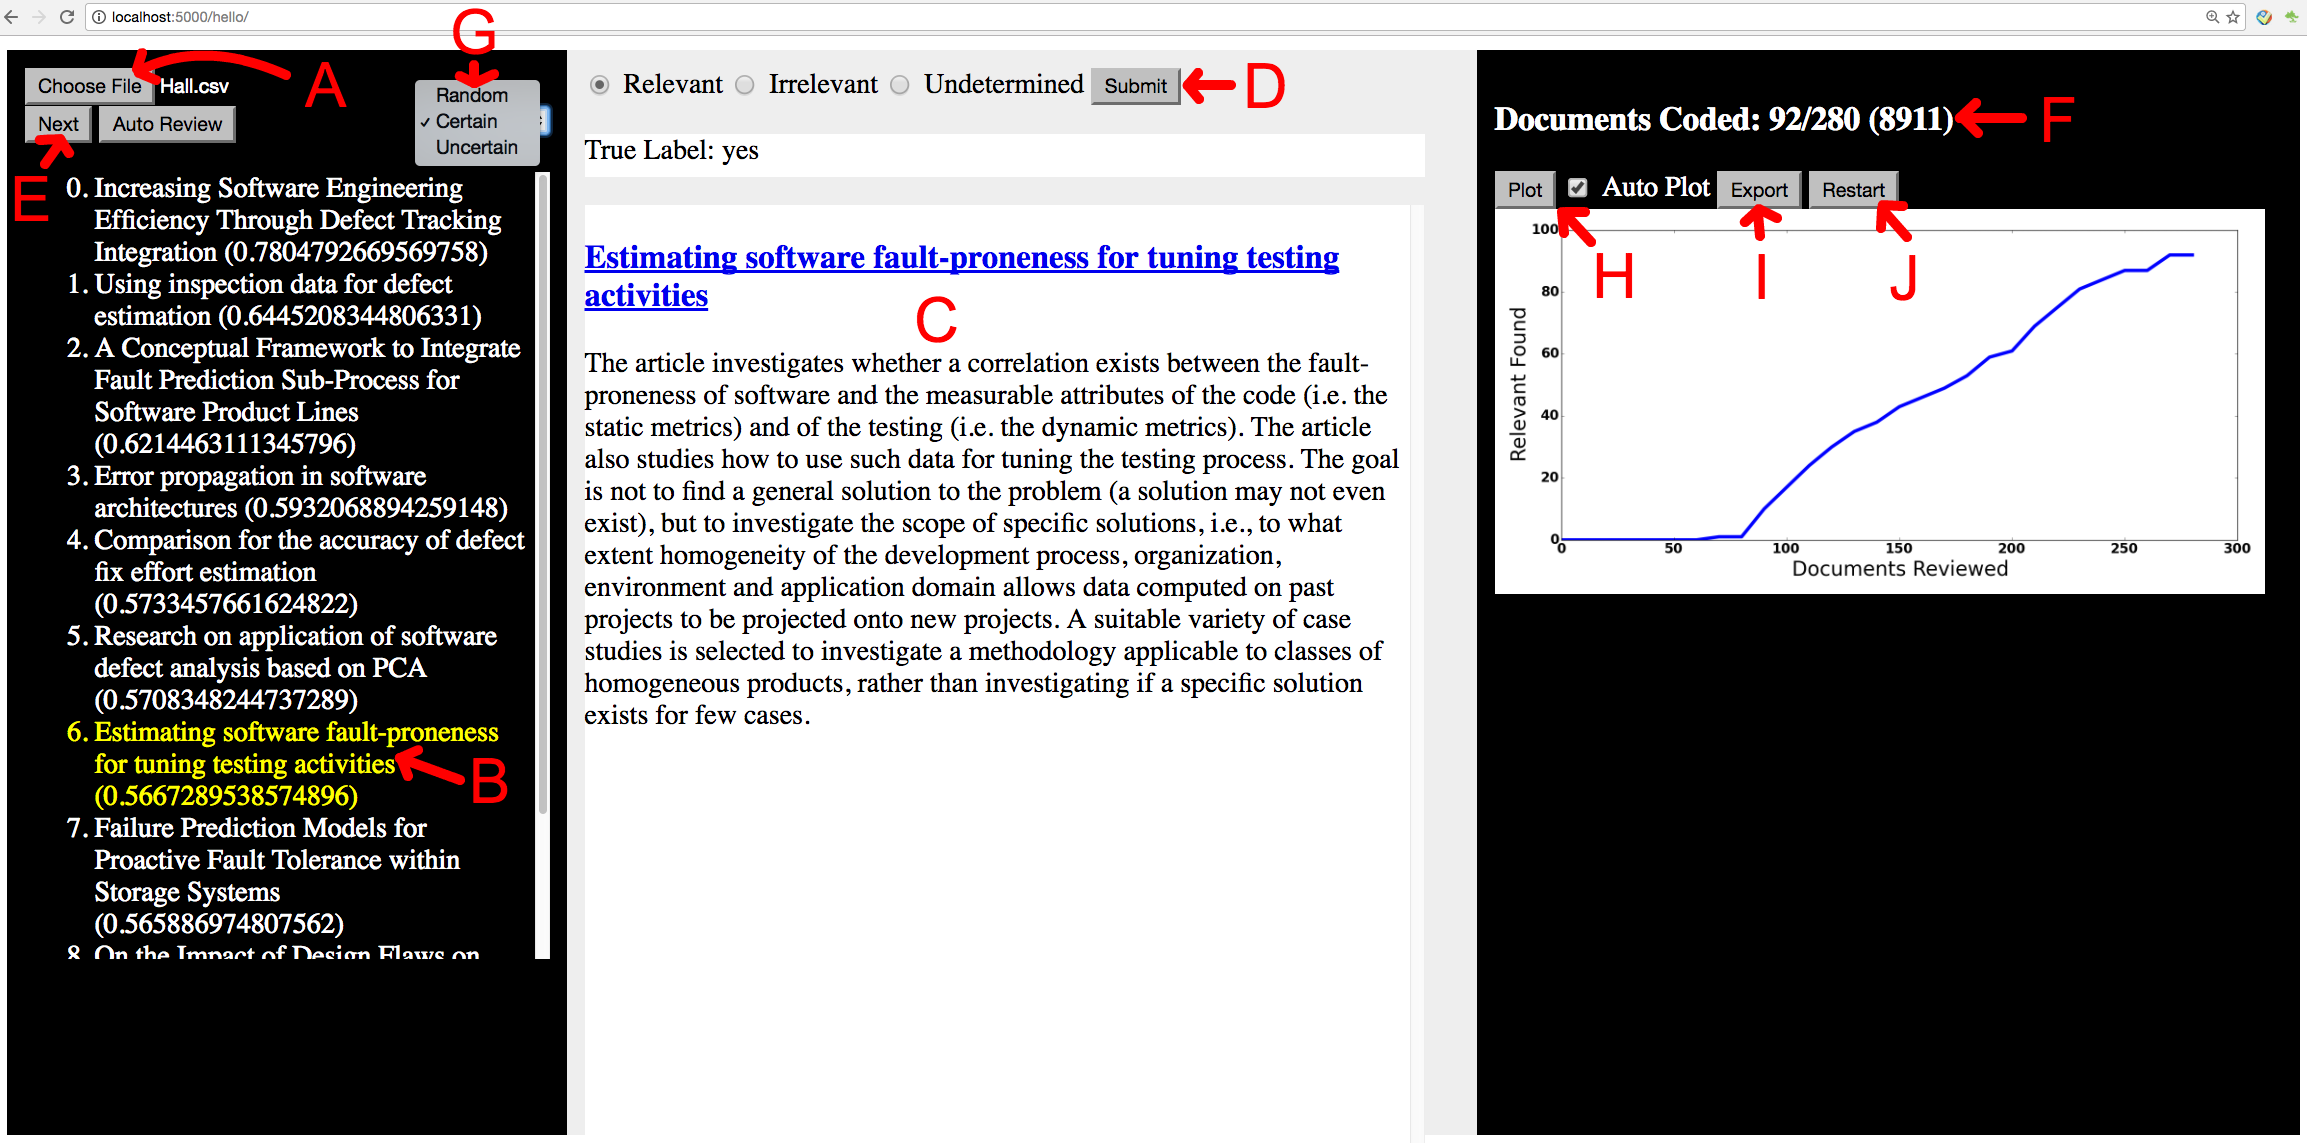
\includegraphics[width=\linewidth]{MAR.png}
    \caption{The MAR tool to implement FASTREAD.}
    \label{fig:MAR}
\end{figure*}

\section{Tool Support}
\label{sect: tool}

In order to implement FASTREAD, we developed a simple tool called MAR, as shown in Figure~\ref{fig:MAR}. This software is freely available
from SeaCraft, Zenodo at \textit{https://doi.org/10.5281/zenodo.192852} and its Github repository at \textit{https://github.com/ai-se/MAR}. 


Using MAR, a FASTREAD review starts with \textbf{A}: selecting the input candidate study list from \textit{MAR/workspace/data/} directory. The input candidate list is specified in the format shown in Figure~\ref{fig:input}. The input CSV file must have the \textit{Document Title}, \textit{Abstract}, \textit{Year}, and \textit{PDF Link} columns. The \textit{label} column, which is the true label of the candidate studies, is optional and is only used for testing. The output CSV file generated by the MAR tool has an additional \textit{code} column, which is the reviewer-decided label for the candidate study. The final inclusion list can be retrieved by extracting all the studies with ``yes'' in the \textit{code} column.

Using MAR, the review then proceeds as follows:
\begin{enumerate}
\item[\textbf{B}] Randomly select $10$ candidate studies for review.
\item[\textbf{C}] Read through the title and abstract (perhaps also click on the title and read the full text) of the candidate study.
\item[\textbf{D}] Decide whether this study should be coded as \textit{Relevant} or \textit{Irrelevant} and click the \textit{Submit} button.
\item[\textbf{E}] Click the \textit{Next} button and the codes are saved. Another $10$ candidate studies will be selected for review.
\item[\textbf{F}] The review status will change every time new studies are coded by reviewer and the \textit{Next} button is hit. The status is shown in the format ``Documents Coded: \textit{Number of relevant studies found} / \textit{Number of studies reviewed} (\textit{Total number of candidate studies}).''
\item[\textbf{G}] Once \textbf{ONE} ``relevant'' study is coded, \textit{Random sampling} can be changed to \textit{Certainty sampling}, as FASTREAD suggests.
\item[\textbf{H}] Figure can be plotted by clicking the \textit{Plot} button or checking \textit{Auto Plot}. The generated figure can also be found in the \textit{MAR/src/static/image/} directory. The new figure will overwrite any old one.
\item[\textbf{I}] Once finished, coded studies can be exported into a CSV file in the \textit{MAR/workspace/coded/} directory, in the format shown in Figure~\ref{fig:output}.
\end{enumerate}

Note that the \textit{Restart} button (\textbf{J}) is only for testing and discards all codes.

\begin{figure}[ht]
    \centering
    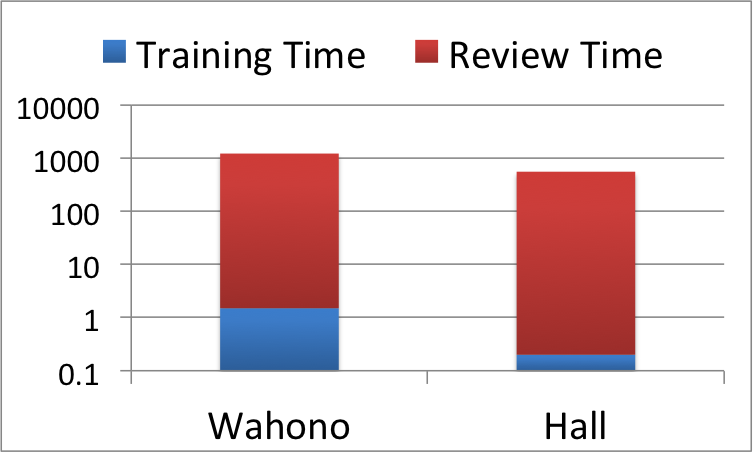
\includegraphics[width=.7\linewidth]{runtime.png}    
    \caption{Runtime cost to achieve $90\%$ recall, measured in minutes, logarithmic scale. The review time in red is estimated as 3 hours for every 100 studies~\cite{malheiros2007visual}.}
    \label{fig:runtime}
\end{figure}

The only extra cost imposed by MAR is training time. The total training time is $13.4$ seconds for Hall data set and $93.1$ seconds for Wahono data set. As demonstrated in Figure~\ref{fig:runtime}, the training time is negligible comparing to review time.



\section{Discussion}

\subsection{Threats to Validity}
\label{sect: Threats to Validity}

There are certain biases that can affect the final
results in this work as with any empirical study. Therefore, any conclusions made from this work must be considered with the following issues in mind:


\subsubsection{Sampling Bias}

sampling bias is a bias in which a sample is collected in such a way that some members of the intended population are less likely to be included than others. Sampling bias threats the results when they are generalized beyond the current scope of study.

All the conclusions in this study are drawn from the experiments running on two software engineering SLR ``gold sets'' generated from Hall, Wahono et al. studies~\cite{hall2012systematic,wahono2015systematic}. Therefore, such conclusions may not be applicable to data sets of different scenarios, e.g., citation screening from evidence based medicine or TAR from e-discovery.

Another place where sampling bias threatens the validity of these results is that both
the ``gold sets'' used in this study extract data from only one data source. Exploration for multiple data sources is left for future work. 

Such sampling biases threatens any classification experiment. The best any researcher can do is document that bias then make available to the general research community all the materials used in a study (with the hope that other researchers will explore similar work on different data sets). Existing machine assisted reading techniques in citation screening have been criticized by by Olorisade et al. for being not replicable~\cite{olorisade2016critical}. To this end, we have published all our code at \textit{https://github.com/ai-se/MAR} and all our data at \textit{https://doi.org/10.5281/zenodo.192506}.

\subsubsection{Learner bias}

Learner bias threats the results with biased selection of learner settings.

The comparisons in our experiment are based on the controlled variables listed in Section~\ref{subsect: Controlled Variables}. These controlled variables are suggested and justified in \cite{krishna2016bigse} as the best practice and lay down the foundation of comparisons. The conclusion in Section~\ref{subsect: Results} may become unreliable if any of the controlled variables changes.

\subsubsection{Evaluation bias}

Evaluation bias may be introduced when one specific evaluation method is preferred.

In this study, \textbf{Recall} vs. \textbf{studies reviewed} curve is utilized to evaluate the performance of each method, as stated in Section~\ref{subsect: Performance Metrics}. It is believed to best fit the objective of machine assisted primary study most~\cite{tredennick2015,cormack2015autonomy,cormack2014evaluation}. The conclusion and result may be different if a different performance metrics is adopted. Further investigation of such metrics is left for future work.

\subsubsection{Order bias}

Order bias is a survey bias by which responses can be affected by the order of answer choices.

The order in which the human reviewer is presented with the candidate studies can affect the results, especially in the random sampling step. To mitigate this order bias, we run the experiment 30 times, randomly changing the order of random sampling and linear review,  and we collect the medians and different percentiles for comparison of both average performance and variance.

\subsubsection{Input bias}

Input bias concerns about the misuse of the input data.

As described in Section~\ref{subsect: Learning based Primary Study Selection}, we assume that the human reviewer is always correct. In practice, this assumption may not hold and problems such as disagreement between reviewers or concept drift (in which reviewers disagree with themselves as time passes) may occur.  As discussed
below when we discuss {\em Future Work}, we intend to explore this matter in the near future.

\section{Conclusions and Future Works}
\label{sect: Conclusion}

Systematic literature reviews are the primary method for aggregating evidence in evidence-based software engineering. It is suggested for every researcher in software engineering to frequently conduct SLRs in~\cite{keele2007guidelines}. The hugest barrier for accomplish this is the cost. Usually an SLR would take months to finish and the conclusion drawn can be out of date in a few years. To tackle this barrier, this study focuses on primary study selection, one of the most difficult and time consuming steps in an SLR, trying to reduce the effort required. Two state-of-the-art machine assisted reading methods, one from evidence-based medicine and one from e-discovery, are refactored for an better method, FASTREAD, to support primary study selection. In our experiments, FASTREAD is capable to retrieve $90\%$ of the ``relevant'' studies by reviewing only $10\%$ of the candidate studies, which means a $90\%$ cost reduction.

This work has lead to a simple software tool called MAR, which
we described above in Section~\ref{sect: tool}. We are currently advertising
that tool on social media and hope that, very soon,
we will be  able to report on
case studies when other researchers use this tool. MAR is
an open source tool, published in Github, and we also hope
that MAR will be maintained and improved by numerous 
researchers exploring this kind of technology. 

This study has several limitations as described in Section~\ref{sect: Threats to Validity} and due to the strict restrictions we place on the scenario in Section~\ref{subsect: Learning based Primary Study Selection}. We plan to address the threats to validity and to loosen those restrictions in future work. Specific problems and plans for the future include:

\begin{itemize}

\item
{\bf Conclusions are drawn from only two SLR data sets with only one data source, which may incur sampling bias.} Validate the results from multiple data sources, on different data sets, including data sets from evidence-based medicine and e-discovery.

\item
{\bf Experiment results are evaluated by \textbf{Recall} vs. \textbf{studies reviewed} curve, which may incur evaluation bias.} Possibilities of other performance metrics will be explored in future work.

\item
{\bf About $10\%$ to $20\%$ efforts are spent on random selection step and most of the variances are also introduced in this step.} To speed up the random selection step, external expert knowledge will be introduced while unsupervised learning methods such as VTM will also be considered in future work. 

\item
{\bf Some of the magic parameters are arbitrarily chosen, which may affect the performance.} For example the margin threshold to determine whether SVM is already stable in uncertainty sampling, the minimum number of ``relevant'' examples to start aggressive undersampling, and when to stop the whole process.

\item
{\bf Current scenario is restricted to having only one reviewer, which is impractical in practice.} Problems including how to assign review tasks to multiple reviewers and how to utilize reviewers with different cost and different capability will be explored in the future.

\item
{\bf Current scenario assumes that reviewers never make mistakes, which is definitely not true in practice.} How to tackle concept drift (reviewers disagree with themselves) and how to settle disagreements (reviewers disagree with each other) would be valuable contributions for future work.

\item
{\bf This study focuses only on primary study selection.} Assists on other steps of SLR such as searching, data extraction, and protocol development can also help to reduce total effort of SLRs. The potential of combining VTM with FASTREAD for a better understanding of the selected primary studies needs to be explored as well.

\end{itemize}

With all the works in this study, a baseline result for learning based primary study selection has been set up. There are plenty of works required to further assist researchers conducting SLRs. However we believe that the effort required for conducting SLRs can be reduced to days of work ultimately and thus enable researchers to conduct SLRs much more frequently.

	\section*{Acknowledgements}
		The work is partially funded by NSF  awards \#1506586 and \#1302169. Thanks are due to Manuel Dominguez for all his
		patient guidance to the legal text mining literature.

%\section*{Acknowledgments}
%Blablabla
 
\vspace*{0.5mm}
 
 
% \bibliographystyle{plain}
\bibliographystyle{elsarticle-num}
% \balance
\bibliography{sigproc} 
% \bibliography
\balance




% that's all folks
\end{document}


